\documentclass{article}

\usepackage[utf8]{inputenc}
\usepackage{amsmath} 
\usepackage{amsfonts}
\usepackage{graphicx}
\usepackage{tabularx}
\usepackage{array}
\usepackage{booktabs}
\usepackage{listings}
\usepackage{hyperref}

% Multiple plots.
%\usepackage[demo]{graphicx}
\usepackage{subcaption}


% Bibliography:
\usepackage[style=authoryear]{biblatex}
\addbibresource{references.bib}
% To compile:
% pdflatex main.tex
% biber main
% pdflatex main.tex
% pdflatex main.tex

% Graphics: 
\graphicspath{ {./output/} }
\usepackage{float} % to force location of pictures, use "H"

% Author and Title:
\author{Paulo Gugelmo Cavalheiro Dias}
\title{Master Thesis: Climate change economic effect on health through temperature}

\begin{document}


\maketitle

\newpage
\tableofcontents

\newpage
\section{Introduction}
Temperature is a fundamental component of the
physical environment, shaping human activity
across multiple dimensions. As climate change
alters the global distribution of temperature,
there is growing concern about its broader
economic consequences. While substantial
attention has been given to the direct effects
of temperature on labor productivity,
agricultural yields, and conflict, less
is understood about how temperature-driven
changes in health may propagate through the
economy over the long run.

Health is a critical input into individual
well-being and economic performance.
Variations in temperature can influence
the incidence and severity of disease,
the functioning of the human body, and
the demand for medical services. These
effects, in turn, may alter labor supply,
human capital accumulation, and lifetime
income trajectories. Understanding the
economic cost associated with these health
effects is essential for quantifying the
full burden of climate change and for
informing effective adaptation policy.

\subsection{Related literature}

This paper contributes to three main strands of literature: health economics, the economics of climate change, and the intersection of climate and health. Each of these fields provides foundational insights but leaves open important questions regarding the long-run economic consequences of temperature-induced health variation.

\subsubsection{Health Economics}

A large literature has documented the central role of health
in shaping economic behavior over the life cycle.
De Nardi et al. (2023) demonstrate that health status
significantly affects labor supply, retirement decisions,
and savings dynamics, establishing health as a key determinant
of productivity and economic welfare.
Beyond contemporaneous productivity effects,
poor health imposes substantial intertemporal costs.
Both De Nardi et al. (2023) and Capatina (2015) quantify
the lifetime income and utility losses associated with
adverse health trajectories, emphasizing the compounding
nature of health shocks over the life course.

\subsubsection{Climate and Economics}

The economic impacts of climate change are multifaceted, with temperature emerging as a particularly influential channel. Burke et al. (2015) document substantial aggregate output losses associated with rising temperatures, particularly in countries with limited adaptive capacity. More recently, Bilal and Kanzig (2024, 2025) show that temperature shocks have asset-pricing implications, underscoring the forward-looking nature of climate risks.

At the same time, the literature has explored how extreme heat may exacerbate social and political instability. Burke, Hsiang, and Miguel (2015) provide compelling evidence that hotter temperatures increase the likelihood of conflict in developing countries, suggesting that the consequences of climate change extend well beyond output measures. Importantly, adaptation has been shown to significantly mitigate the economic burden of climate shocks. Carleton et al. (2022) estimate the global mortality consequences of warming while explicitly accounting for adaptation costs and benefits, illustrating how policy and behavioral responses shape climate damages.

From a methodological standpoint, the empirical identification of climate impacts presents persistent challenges. Deryugina and Hsiang (2017), Hsiang (2016), and Nordhaus (2019) all highlight the difficulties of isolating causal effects in the presence of spatial and temporal heterogeneity. Bilal and Kanzig (2024, 2025) further emphasize the econometric complexity involved in measuring forward-looking responses to climate risks.

\subsubsection{Climate and Health}

A growing body of work links temperature variation to health outcomes. Barreca et al. (2016) show that the temperature-mortality relationship in the U.S. has declined substantially over the twentieth century, pointing to significant adaptation in developed economies. Nevertheless, the potential for major health shocks remains. The IPCC (2022, Chapter 7) outlines the anticipated health risks under various warming scenarios, concluding that climate-related health burdens are likely to intensify even in high-income countries.

\subsubsection{Gap in the Literature}

While prior research has examined the contemporaneous
effects of temperature on economic output, and others
have quantified the cost of poor health on lifetime
economic outcomes, little is known about how
temperature-induced health variation translates
into long-run income losses at the individual level.
Moreover, existing work often abstracts from or aggregates
over individual responses.

This Master Thesis addresses this gap by quantifying
the lifetime economic cost of temperature-driven health
deterioration in the context of the USA,
under current levels of adaptation and within a
structural life-cycle framework of individual decision-making.

\subsection{Research question and strategy}

The economic consequences of temperature-induced health variation reflect a fundamental tradeoff embedded in individual decision-making. Higher temperatures can deteriorate health outcomes, impairing both physical capacity and cognitive functioning, which in turn depresses labor productivity and expected longevity. These changes can have long-lasting effects on income profiles, particularly when health deteriorates early in life.

Yet even in the absence of institutional responses or targeted health investments, individuals may adjust their economic behavior in response to deteriorating health. A worsening health trajectory may lead agents to reoptimize by altering labor supply, savings, or consumption paths. These behavioral responses—though constrained—can partially absorb the economic shock. The key question is then whether such individual adjustments are sufficient to mitigate the lifetime income loss induced by temperature-related health shocks, or whether the long-run economic cost remains substantial despite endogenous reoptimization.

This tension motivates the central research question of this paper:
How do temperature-induced health shocks affect individuals’ lifetime income, when only individual-level behavioral responses are allowed, and what are the economic mechanisms through which these effects propagate?

To address this question, the analysis proceeds in two stages.
First, an empirical investigation quantifies the causal impact of temperature variation on individual health status.
Using micro-level data, the analysis estimates how both short-term and sustained exposure to high temperatures affect health outcomes across demographic groups and age cohorts.

Second, these empirical estimates are embedded into a structural, life-cycle model of individual behavior.
In the model, health enters as a state variable that evolves over time and affects both survival and future health probability distribution.
Individuals maximize lifetime utility by choosing labor supply and consumption paths, taking health dynamics as exogenous but responsive to temperature.
Crucially, the model does not incorporate health investment or collective adaptation, isolating the role of individual optimization.

By simulating the model under alternative temperature scenarios, the analysis computes the long-run income losses attributable to temperature-induced health shocks. These results yield a quantitative assessment of the intertemporal economic cost of climate-related health deterioration, under a benchmark of minimal adaptation.

\section{Setting}

This section is dedicated to the presentation of the general setting
in which individuals live in this model.
First, the relationships between the different elements in a general framework will be presented.
Then, the data used will be presented and discussed. 
The methods used to estimate the functional forms of the relationships will then be 
presented, and will be refered as the specific case of this work.
Finally, results of the estimation process of these relationships will be presented and discussed.

\subsection{Formal Description}

At each period, an exogenous weather realization occurs, and individuals draw a health and living status. 

\subsubsection{History vectors}

In a general framework, we can think of the health of an individual at time $t$ as a vector $\mathcal{H}_t\in \mathbb{R}^{t}$ containing
all the health status of the individual throughout their life.
Similarily, we can think of the weather experienced by an individual at time $t$ as a vector $\mathcal{W}_t\in \mathbb{R}^{t}$ containing
all the weather conditions experienced by the same individual throughout their life.

\subsubsection{Health Status}

Let $H_{t}\in\Omega(H)$ be a random variable denoting the health status of an individual at time $t$.
The functional form of its distribution $f_{h}$ will depend on its sample space $\Omega(H)$. 
The past health history and the temperature also affect the probability distribution of health status.
Generically, we can therefore write: 

\begin{equation}
    H_{t}\sim f_{h}(\mathcal{H}_{t-1},\mathcal{W}_t)
\end{equation}

Also, it follows that: 

\begin{equation}
    \mathcal{H}_{t} = (H_{1},...,H_{t})
\end{equation}

\subsubsection{Living Status}

Let $L_{t}\in\{0,1\}$ be a random binary variable denoting the living status of an individual at time $t$.
It is determined by a Bernoulli distribution with parameter $p_t$ such that: 

\begin{equation}
    L_{t} \sim \mathcal{B}(p_{t})
\end{equation}

The probability parameter $p_{t}$ depends on their health, age, and temperature.
In a general approach, we can rewrite the first equation such as: 

\begin{equation}
    L_{t} \sim \mathcal{B}(p_{t}(\mathcal{H}_t,\mathcal{W}_t))
\end{equation}

% As such, the probability of an individual to be alive at period $t$ is: 
% 
% \begin{equation}
%     Pr(L_t = 1 | \mathcal{H}_t,\mathcal{W}_t ) = \prod_{j = 1}^{t} p_{j}(\mathcal{H}_j,\mathcal{W}_j)
% \end{equation}

\subsection{Data}

Three main datasets were used to estimate these relationships: 
the Health and Retirement Study (HRS) dataset for
health information and survival,
the Berkeley Earth dataset for annual temperature,
and the Federal Reserve Bank of Saint Louis (FRED) dataset for 
other economic variables.

\subsubsection{HRS Data}

The HRS has a main survey performed every two years on a panel of individuals in the United States of America (USA). 
An exit survey occurs in parallel, that targets individuals identified as dead, in which questions are asked to relatives.
The exit survey was used to identify dead individual, for which the living status was noted as $0$ at the year of the survey. 
Dead individuals were kept in the final analyzed dataset if they had been observed in the immediate previous survey. 
To avoid mortality effects of the COVID-19, the latest year selected for this study was 2018.
Due to different encoding, the 2000 and prior surveys were not taken into account. 

Four variables were used in this dataset: Year of the survey, age of individuals, living status, and health status.

The age of individuals was determined based on the year of birth question, that was substracted to the year of the survey. 
Living status was encoded as $1$ if an individuals was present in the main survey, and $0$ if they were in the exit survey.
The health status of dead individuals was encoded as the same as in the previous survey. 
The Health Proxy defined above was constitued by adding four variables,
from the main survey, and obtained by asking individuals if they have had blood pressure,
lung disease, hearth condition, and stroke accidents.
The health status was identified through the self-reported health.
This measure is less precise than alternative composites, based on weighted average of specific questions of health, 
but perform well enough and is more tractable.

In the HRS data, health status can take eight possible values: 


- 1: Excellent

- 2: Very Good

- 3: Good

- 4: Fair

- 5: Poor

- 8, -8, or 9: Non Available, Not answered, or refused to answer\footnote{This last category was removed from the final analyzed dataset.}\\



\begin{figure}[H]
    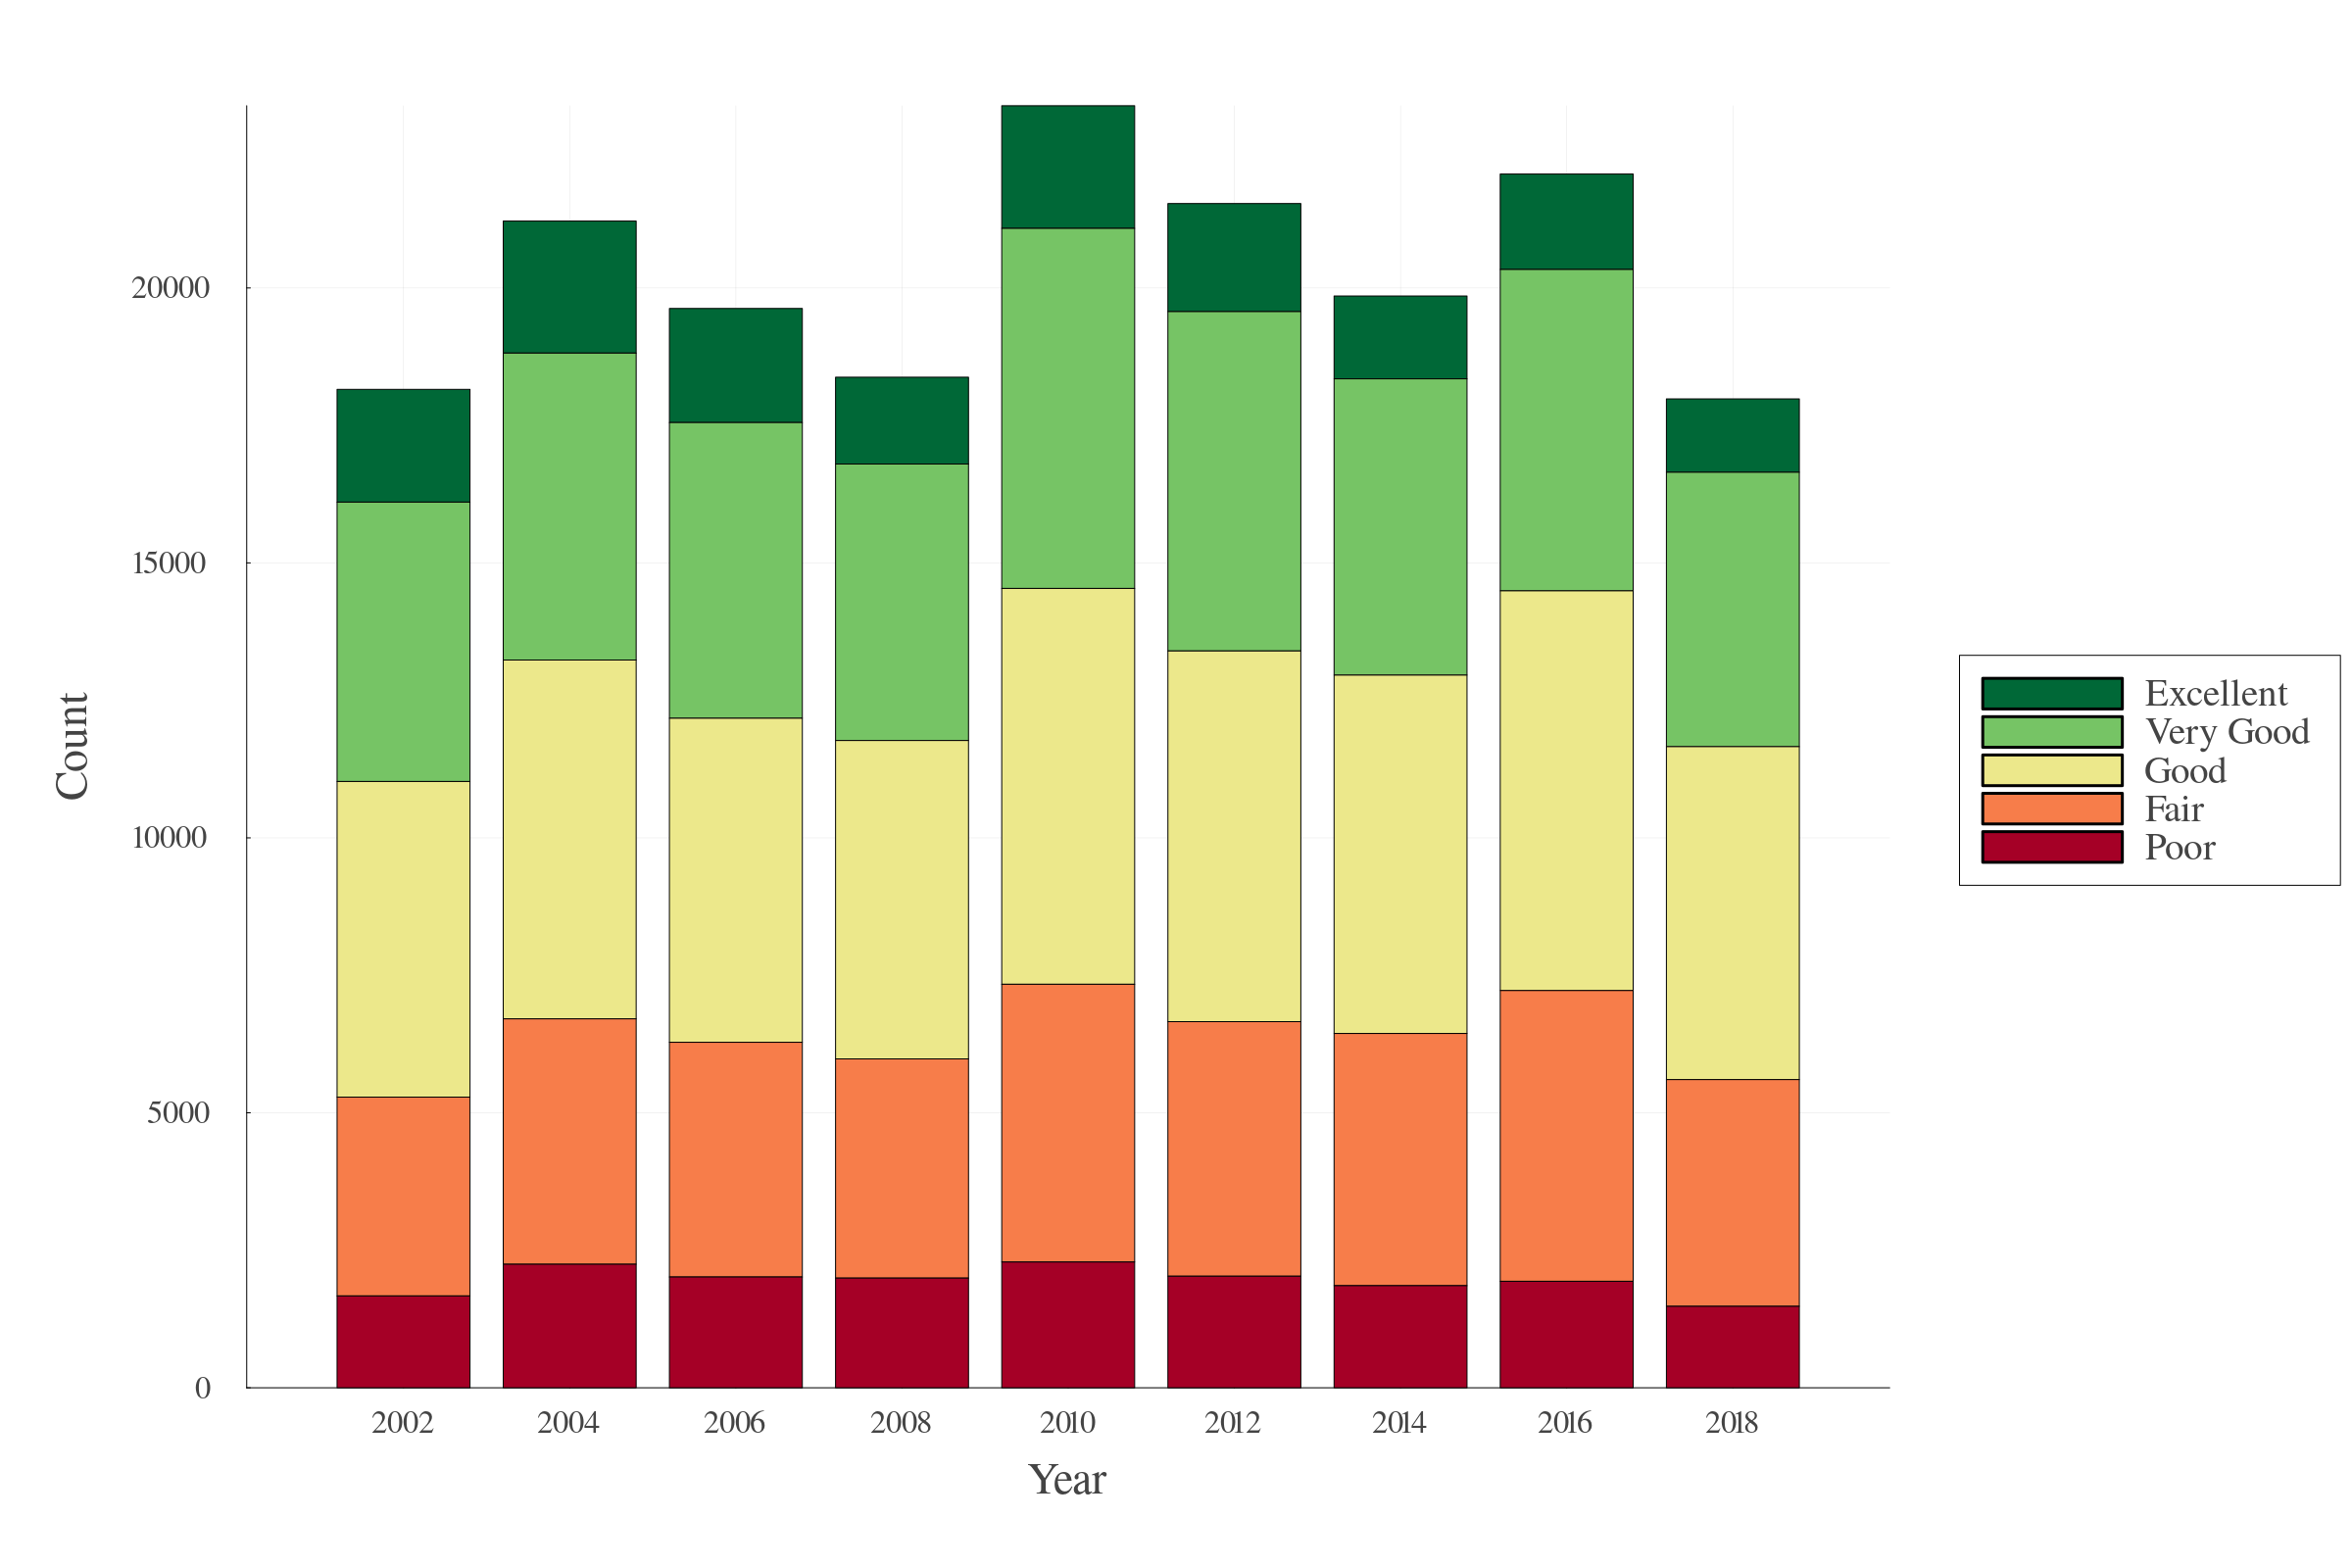
\includegraphics[width=\textwidth]{/Users/paulogcd/Documents/Master_Thesis/working_elements/Draft/output/histogram_1.png}
    \caption{Health Status distribution per Year, from the HRS data}
\end{figure}

\subsubsection{Climate Data}

The climate data of Berkeley Earth was used to collect information
on average annual or pluriannual global temperature on land.
The name of the chosen dataset was the ``Land Monthly Average Temperature''. 
% This file contains a detailed summary of the land-surface average 
% results produced by the Berkeley Averaging method.  Temperatures are 
% in Celsius and reported as anomalies relative to the Jan 1951-Dec 1980 
% average.  Uncertainties represent the 95% confidence interval for 
% statistical and spatial undersampling effects.
For each month, from 1880 to 2022, two anomaly extrema values are given. 
They correspond to the 95\% confidence interval for the
average temperature. 
The average temperature is computed as a deviation from the average annual 
temperature computed between Januray 1951 and December 1980. 

\begin{figure}[H]
    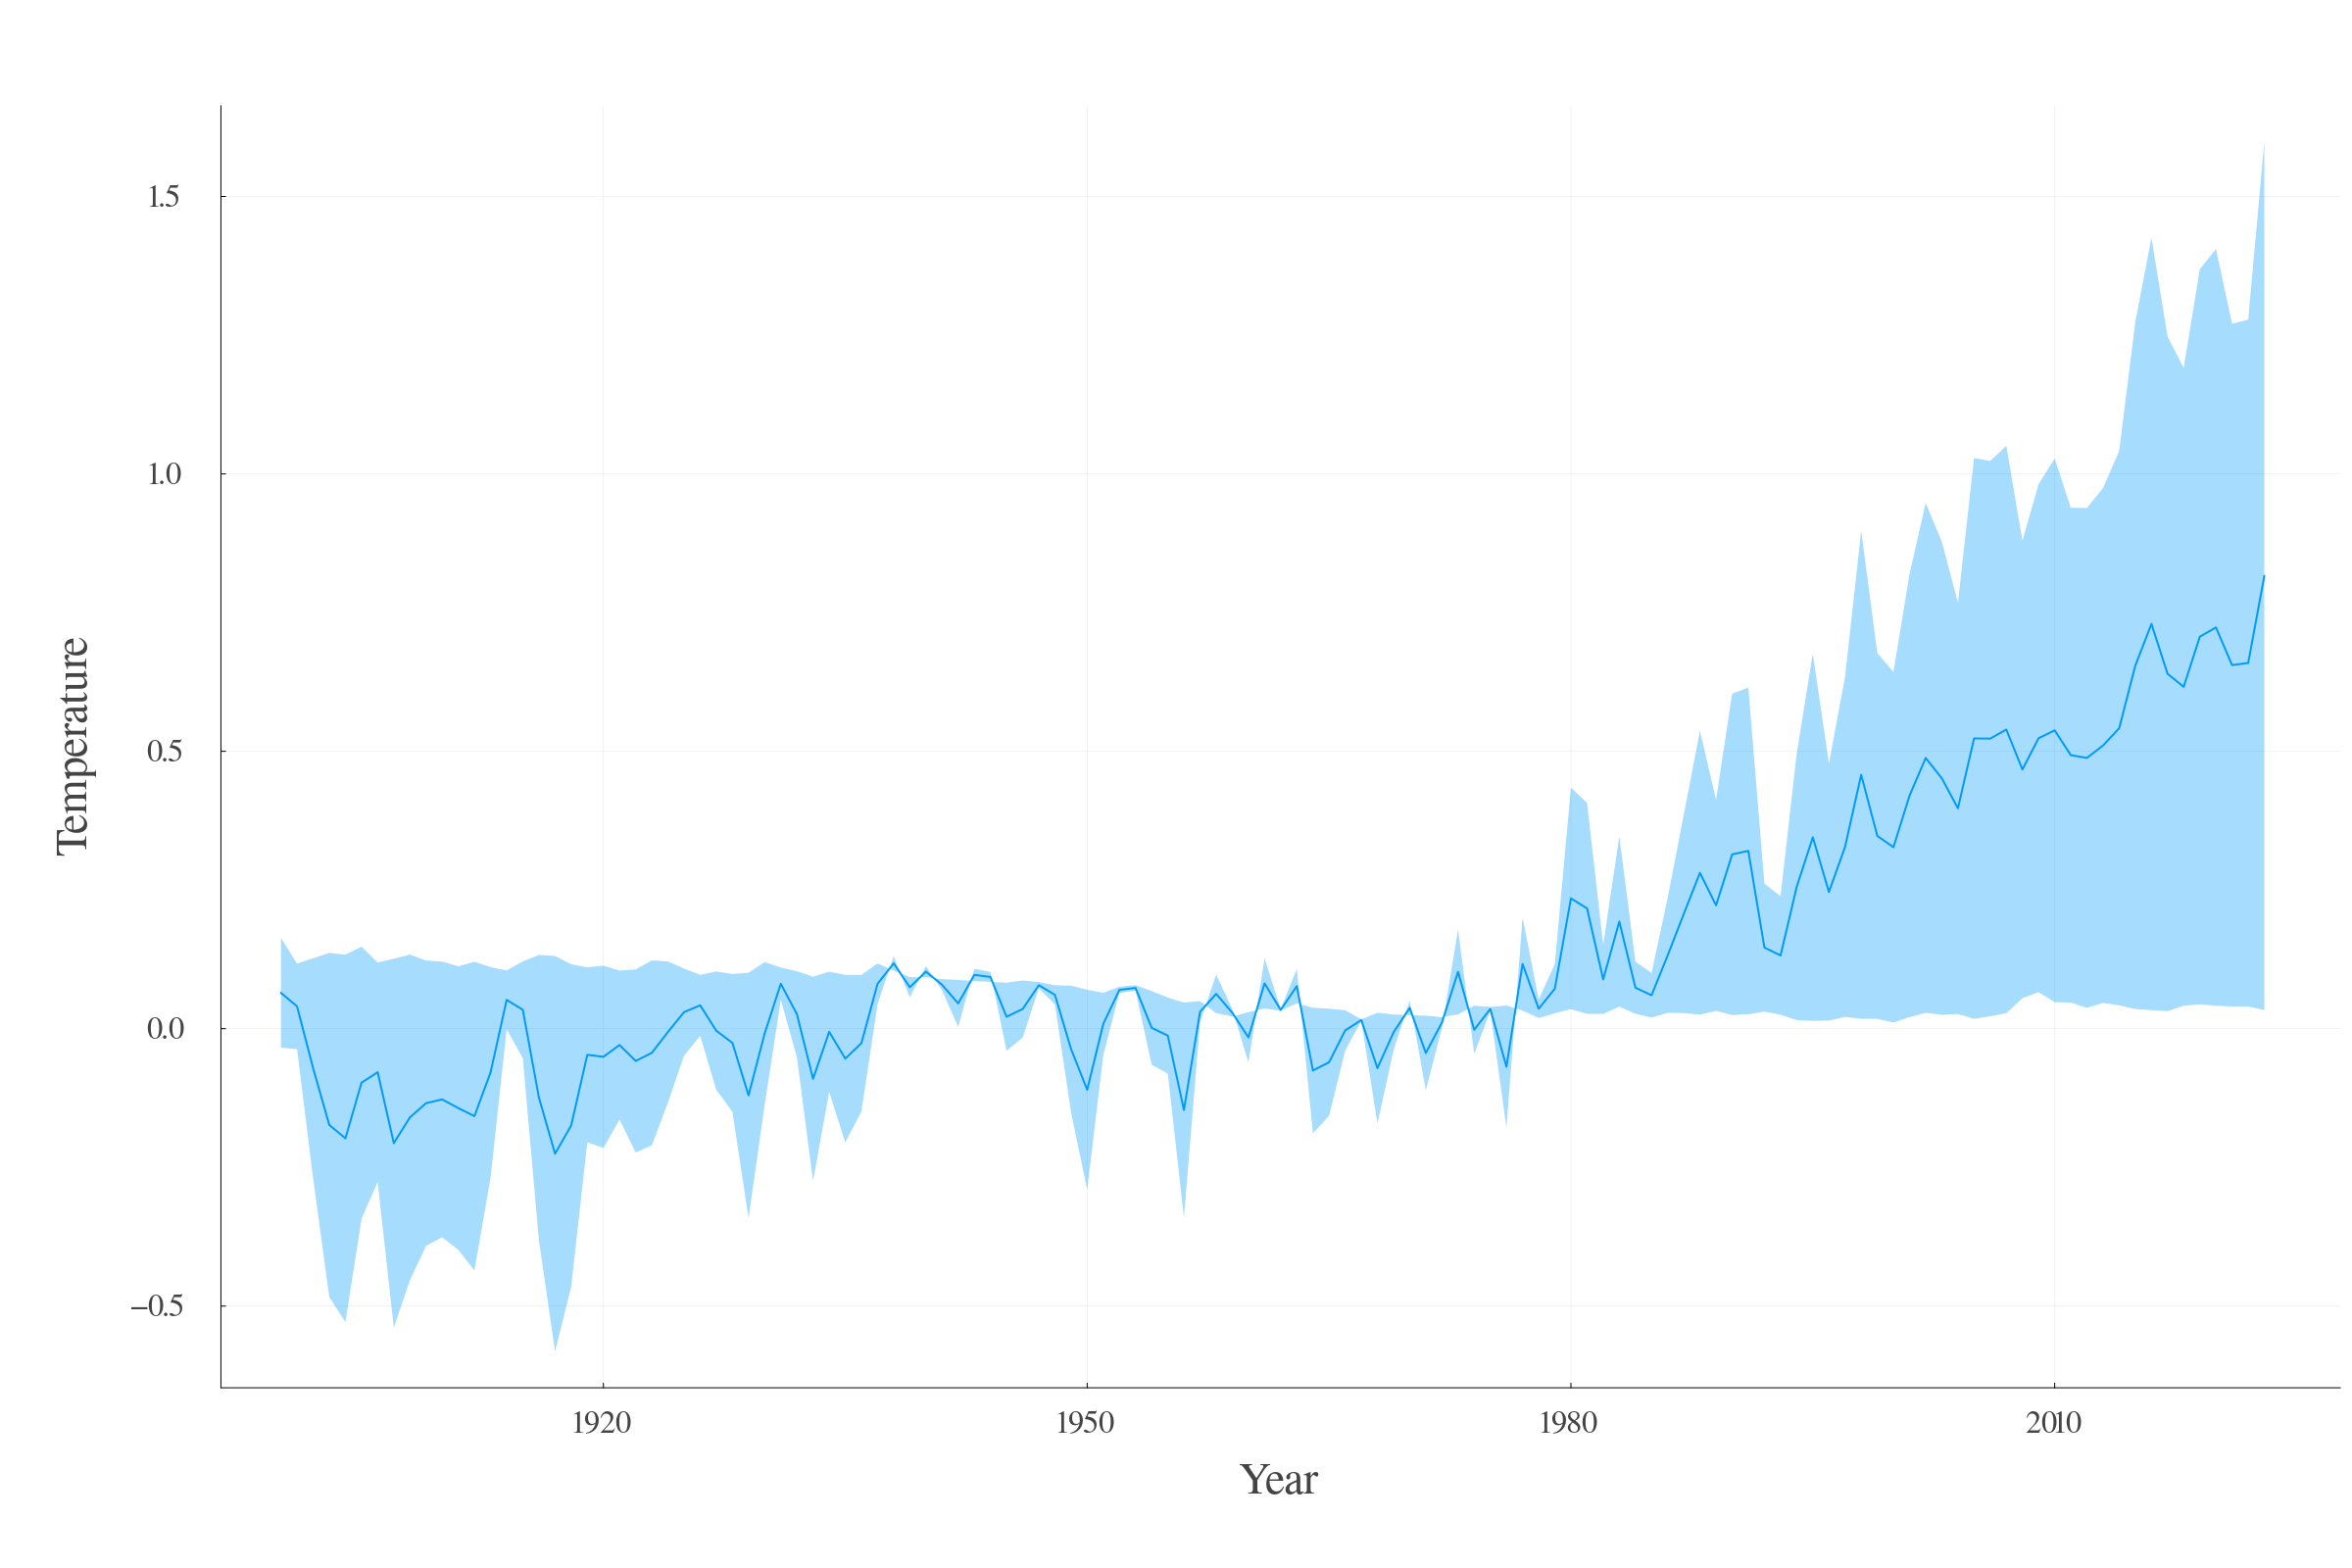
\includegraphics[width=\textwidth]{/Users/paulogcd/Documents/Master_Thesis/working_elements/Draft/output/figure_1.png}
    \caption{Average annual temperature from the Berkeley Dataset}
    
    The light blue area is delimited by the anomalies extrema of each year, and
    the dark blue line represents the average of the anomalies.
\end{figure}

\subsubsection{Economic Data}

Finally, the FRED data was used to get two economic variables. 
First, the annual Gross Domestic Product (GDP) of the USA. 
Second, the interest rate, whose average is then used to calibrate the economic model.

\section{Estimation Methods}

\subsection{Health Transition}

The HRS dataset provides rich information regarding the health status of individuals. 
To make use of the five different values of the self reported health, it was therefore decided not to
recode the variables into a binary health status variable $H\in\{Bad, Good\}$. 

Several methods were considered to estimate the relationship between current health and past health and other covariates. 
Given that health is here an discrete, ordinal variable, ordered response models were chosen.
More specifically, the ordered logit and ordered probit models were selected, due to their simplicity and broad usage \parencite{Wooldridge_2010}.

For tractability and computational reasons, 
it was chosen not to overload the function with 
history parameters, and just to focus on recent health, 
and on current temperature.
Therefore, 
$f_{h}(\mathcal{H}_{t-1},\mathcal{W}_{t})$ 
is considered as $f_{h}(H_{t-1},{T}_{t})$ from now onwards.

Since $\Omega(H_{t}) = [\![1,5]\!]$, we can consider 
$f_{h}$ as a categorical distribution
function\footnote{Also called generalized Bernoulli distribution, that can be represented as a Markov transition matrix.}.
It can therefore be written as: 

\begin{equation}
    f_{h}(H_{t-1} = j,{T}_{t}) = 
    f_{h,j}(T_{t}), \ \forall j\in [\![1,5]\!]
\end{equation}

To estimate $f_{h,j}(T_{t})$,
i.e. the probabilities to go to another health state
given that $H_{t-1} = j$, 
a first naive approach would consist 
in running an ordinal logistic 
regression with $H_{t}$ as the dependent 
variable, and the with covariates including 
the age, temperature, and control variables.

There are two main issues with this regression. 
First, there is a large amount of omitted variables
affecting the survival probability in this formulation.
Second, when we try to include economic variables reflecting 
the progress in medicine, economic development, or 
other kinds of control to take into account possible
omitted variables, 
we are faced with a colinearity issues
with temperature. 

Another important element to take into account to estimate 
$f_{h}(\cdot)$ are the interaction 
effects between the different covariates.
For example, it seems plausible that age and previous health status interact:
Being in ``Fair"
health should not have the same effect on the health transition probability 
for a 20 years old individual compared to a 80 years old individual. 

To tackle these problems, it is possible to use a 
IV-based approach to try to isolate the effect of
temperature on health. 
To do so, let us define a Health Proxy ($HP_{i,t}$) as 
the sum of binary variables at time $t$ for individual 
$i$ indicating if they have health issues.
I retained four possible health accident, 
that can all be related to exposure to 
high levels of ambient temperature, such that: 

$$
    X_{i,t}^{h} =
    \begin{bmatrix}
        \text{High Blood Pressure}_{i,t} \\
        \text{Lung Disease}_{i,t} \\ 
        \text{Hearth Condition}_{i,t} \\ 
        \text{Stroke}_{i,t}
    \end{bmatrix}
$$

Formally, the Health Proxy can therefore be written as:

\begin{equation}
    HP_{i,t} = \sum_{j\in X^{h}_{i,t}} j
\end{equation}

We can thus first run the following linear regression,
to estimate the marginal effect of temperature on health
through the above mentioned health accidents:

\begin{equation}
    \widehat{HP}_{i,t}^{I} =  \widehat{\beta_0} +
    \widehat{\beta_{A}} \cdot Age_{i,t} +
    \widehat{\beta_{T}} \cdot Temperature_{t}
\end{equation}

Once we have the estimate $\widehat{HP}_{i,t}^{I}$, we can
then run a second regression, with the transition probability 
as the dependent variables, and with $H_{i,t-1}$ and 
$\widehat{HP}_{i,t}^{I}$ as covariates.

\subsection{Living Status}

The living status variable, being binary, 
a simple logistic regression was possible. 
%When run on age and health
%status, it finds similar results with the
%rest of the literature. 

%\begin{figure}[H]
%    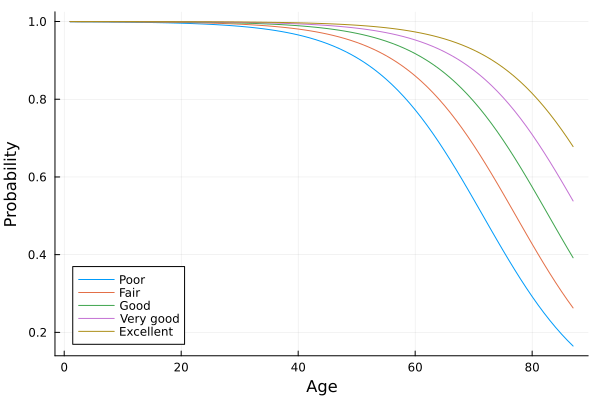
\includegraphics[width=\textwidth]{/Users/paulogcd/Documents/Master_Thesis/working_elements/Draft/output/figure_2.png}
%    \caption{Annual probability of survival as a function of age and health status}
%\end{figure}

To estimate $p_{t}(\mathcal{H}_{t},\mathcal{W}_{t})$,
the first naive approach would have led to the same 
problems as previously seen.
For example, running the non-IV regression with $X$ containing only GDP, 
we find a negative coefficient on temperature, but also with GDP. 
This is due to the recent tendency in the USA in which the life expectancy stays 
stable or decrease slightly, while the GDP continues to raise importantly.

With $\Lambda(\cdot)$ being the logistic
function, we could therefore run the following logistic regression 
to estimate the probability parameter $p_{i,t}$, i.e. the
survival probability of $i$ at $t$,
with the previous estimate $\widehat{HP}_{i,t}^{I}$: 

% \begin{figure}[H]
%     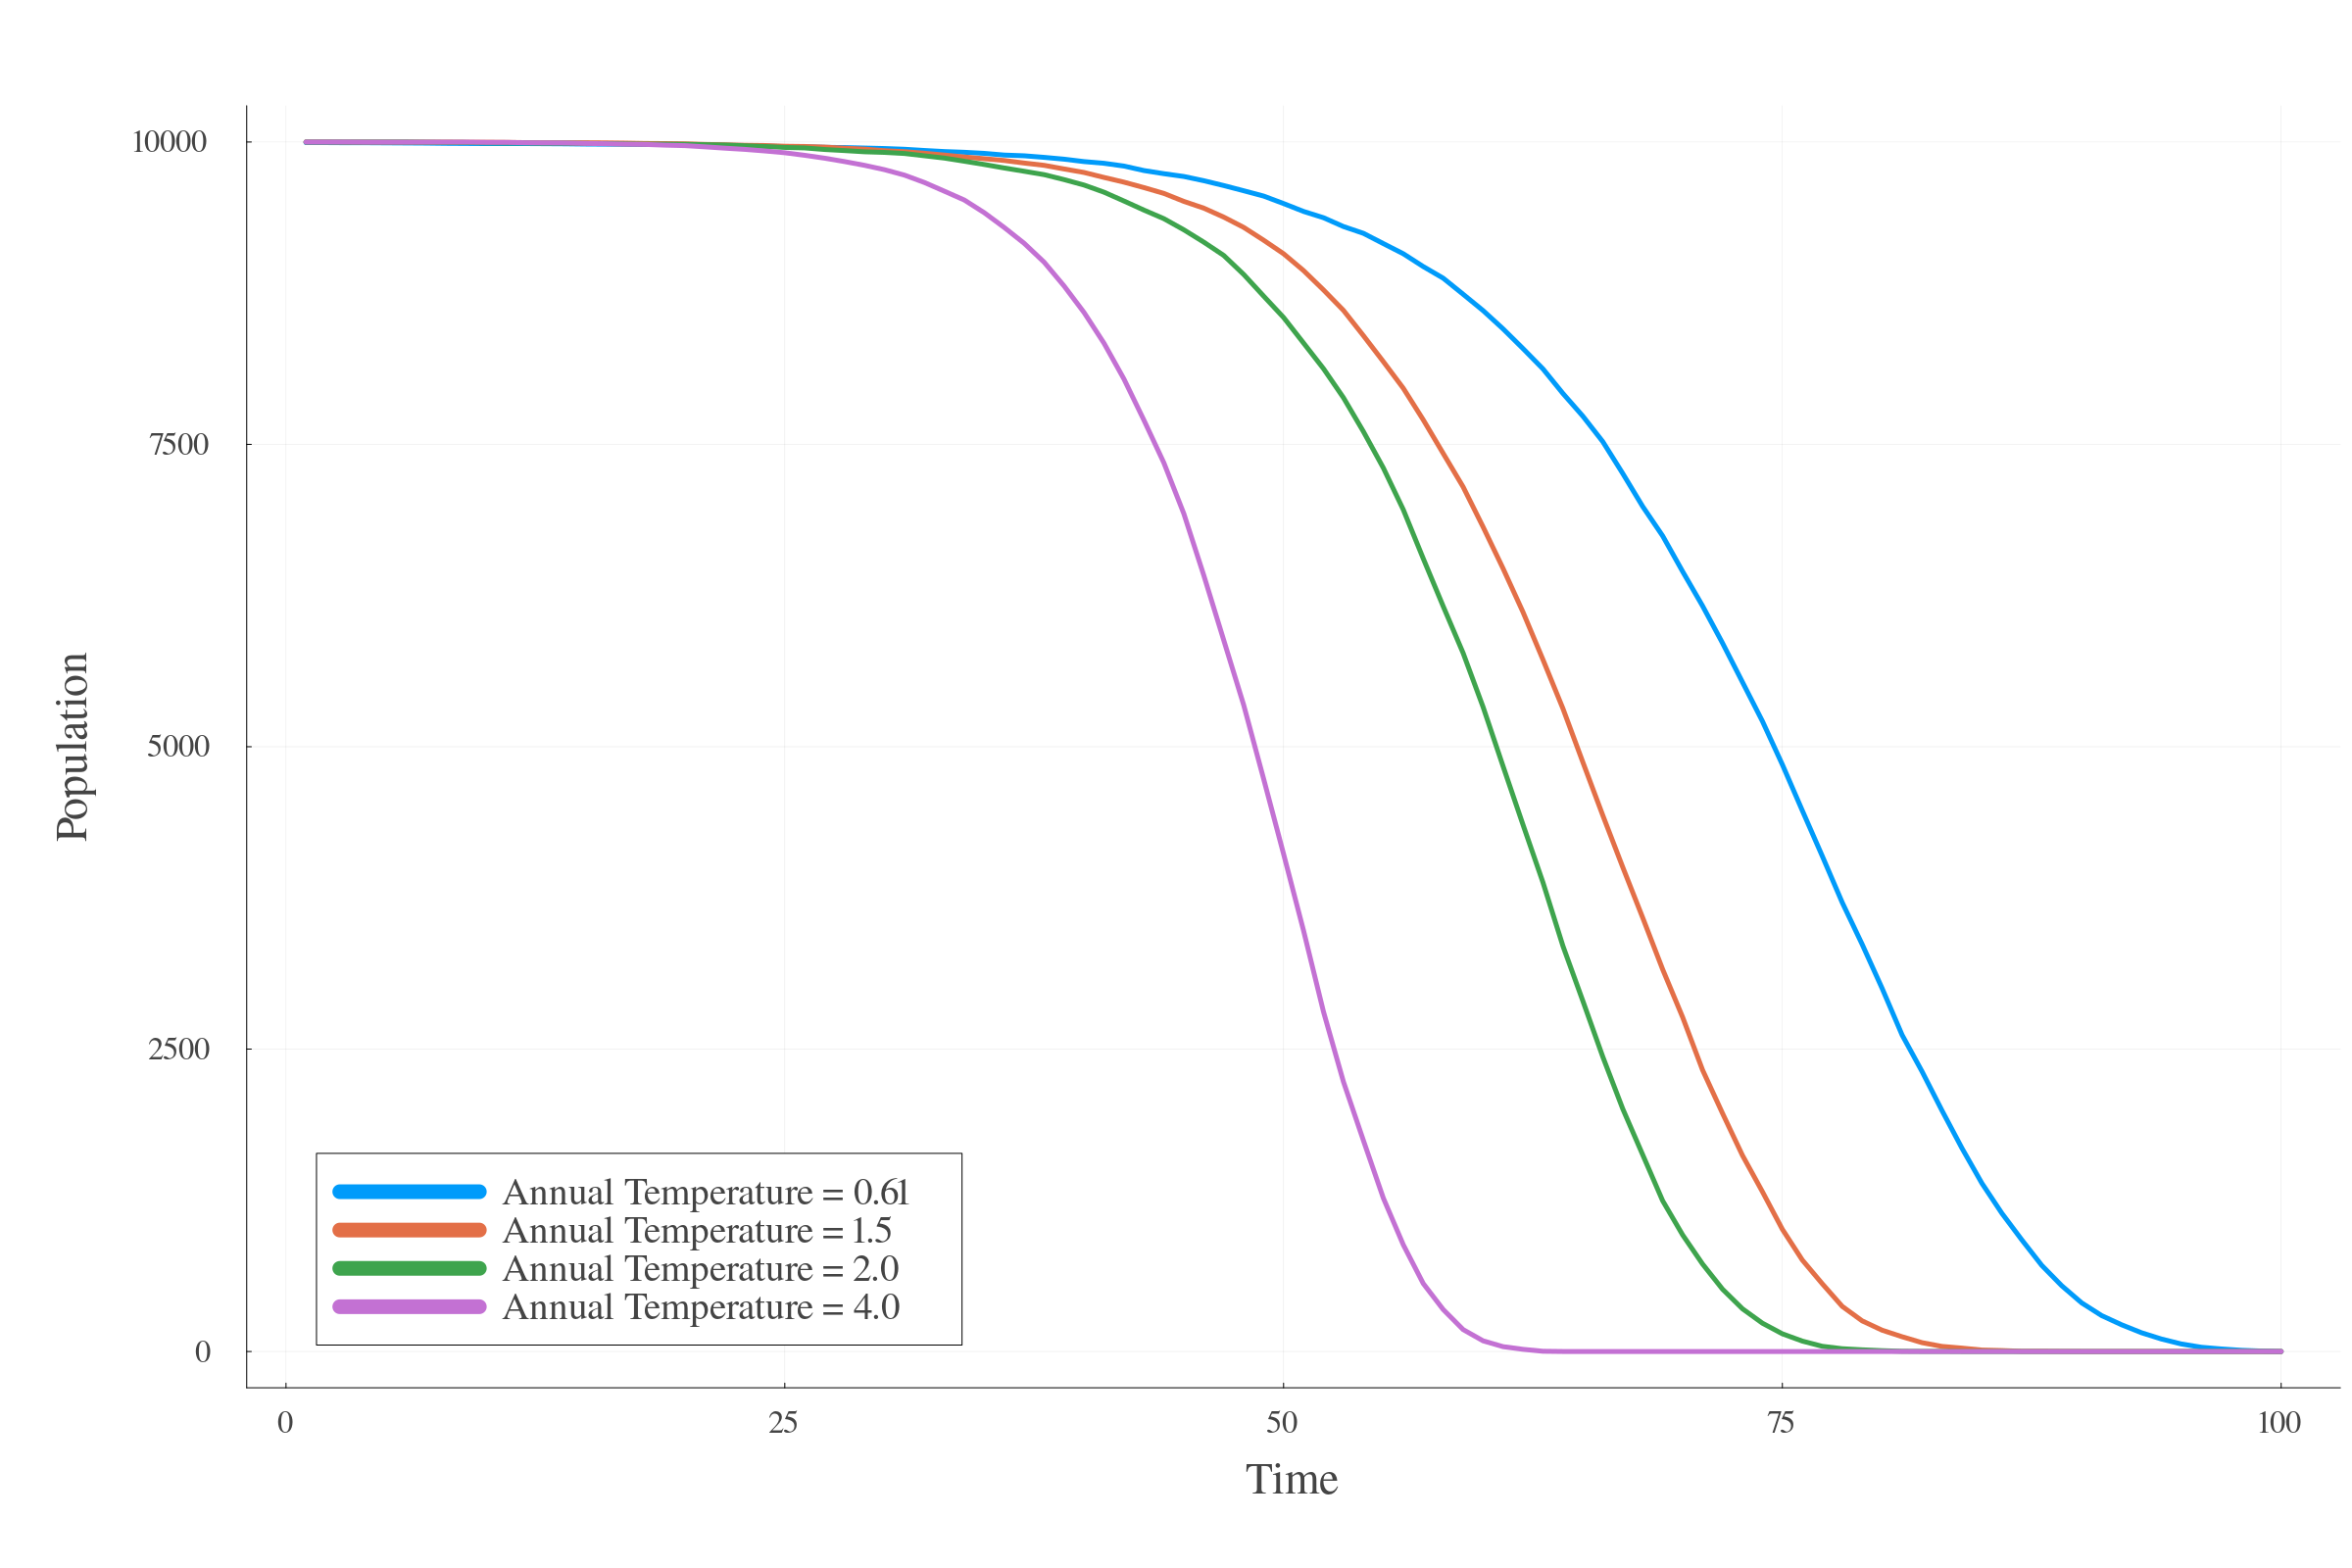
\includegraphics[width=\textwidth]{/Users/paulogcd/Documents/Master_Thesis/working_elements/Draft/output/figure_3.png}
%     \caption{Annual probability of survival as a function of age and health status}
% \end{figure}

\begin{equation}
    \widehat{p_{i,t}} = \Lambda \left( \widehat{\beta_0} +
    \widehat{\beta_{H}} \cdot Health_{i,t} +
    \widehat{\beta_{HP}} \cdot \widehat{HP}_{i,t}^{I}\right)
\end{equation}

\subsection{Estimation Results}

The first regression to explain the Health Proxy yields: 

\begin{table}[H]
    \begin{center}
        \begin{tabular}{lr}
            \toprule
                                    & \multicolumn{1}{c}{HP} \\ 
            \midrule
            (Intercept)              &              -0.487*** \\ 
                                    &                (0.068) \\ 
            Age                      &               0.020*** \\ 
                                    &                (0.001) \\ 
            Temperature              &                 -0.032 \\ 
                                    &                (0.123) \\ 
            Age $\times$ Temperature &                0.005** \\ 
                                    &                (0.002) \\ 
            \midrule
            $N$                      &                182,947 \\ 
            $R^2$                    &                  0.086 \\ 
            \bottomrule
        \end{tabular}
        \caption{Regression of Health Proxy on Age, Temperature, and their interaction.}
    \end{center}
\end{table}

\subsubsection{Health transition}

The regression to estimate the health transition probabilities
yields. 

\begin{figure}[H]
    \begin{subfigure}{.5\textwidth}
    \centering
    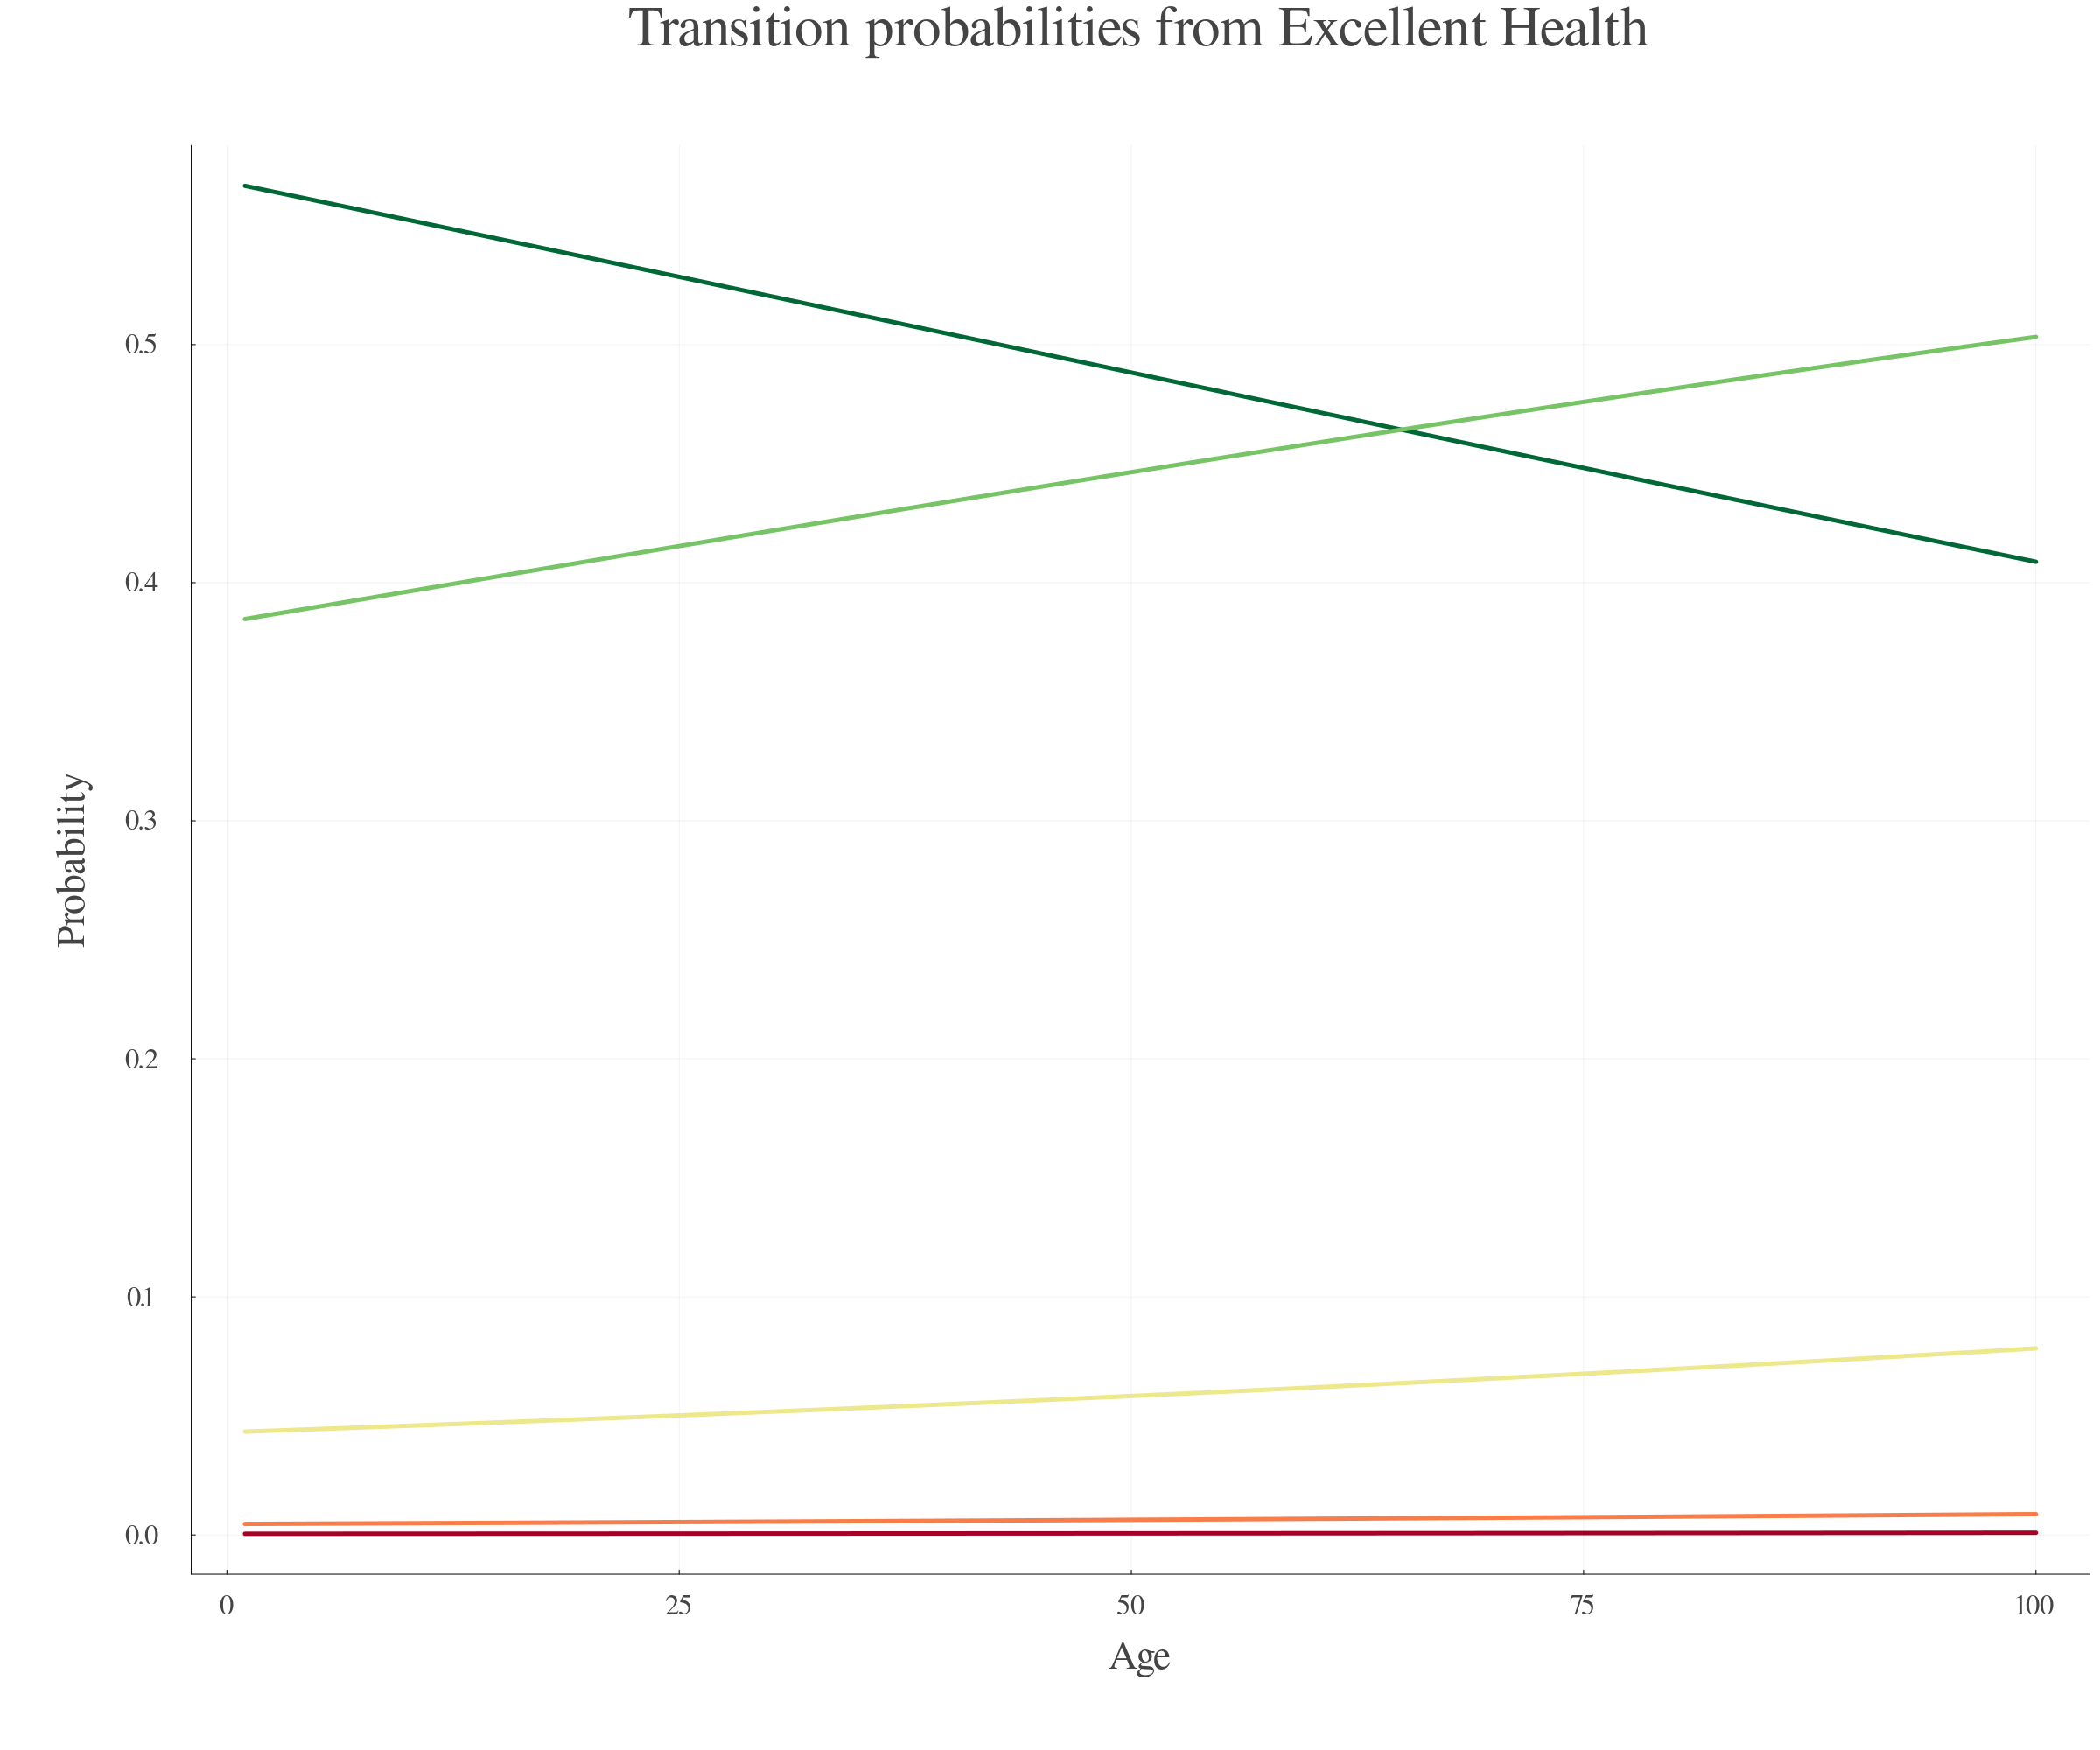
\includegraphics[width=\linewidth]{/Users/paulogcd/Documents/Master_Thesis/working_elements/Draft/output/health_transition_1.png}
    \caption{Transition probabilities from Excellent Health}
    \label{fig:sfig1}
    \end{subfigure}%
    \begin{subfigure}{.5\textwidth}
    \centering
    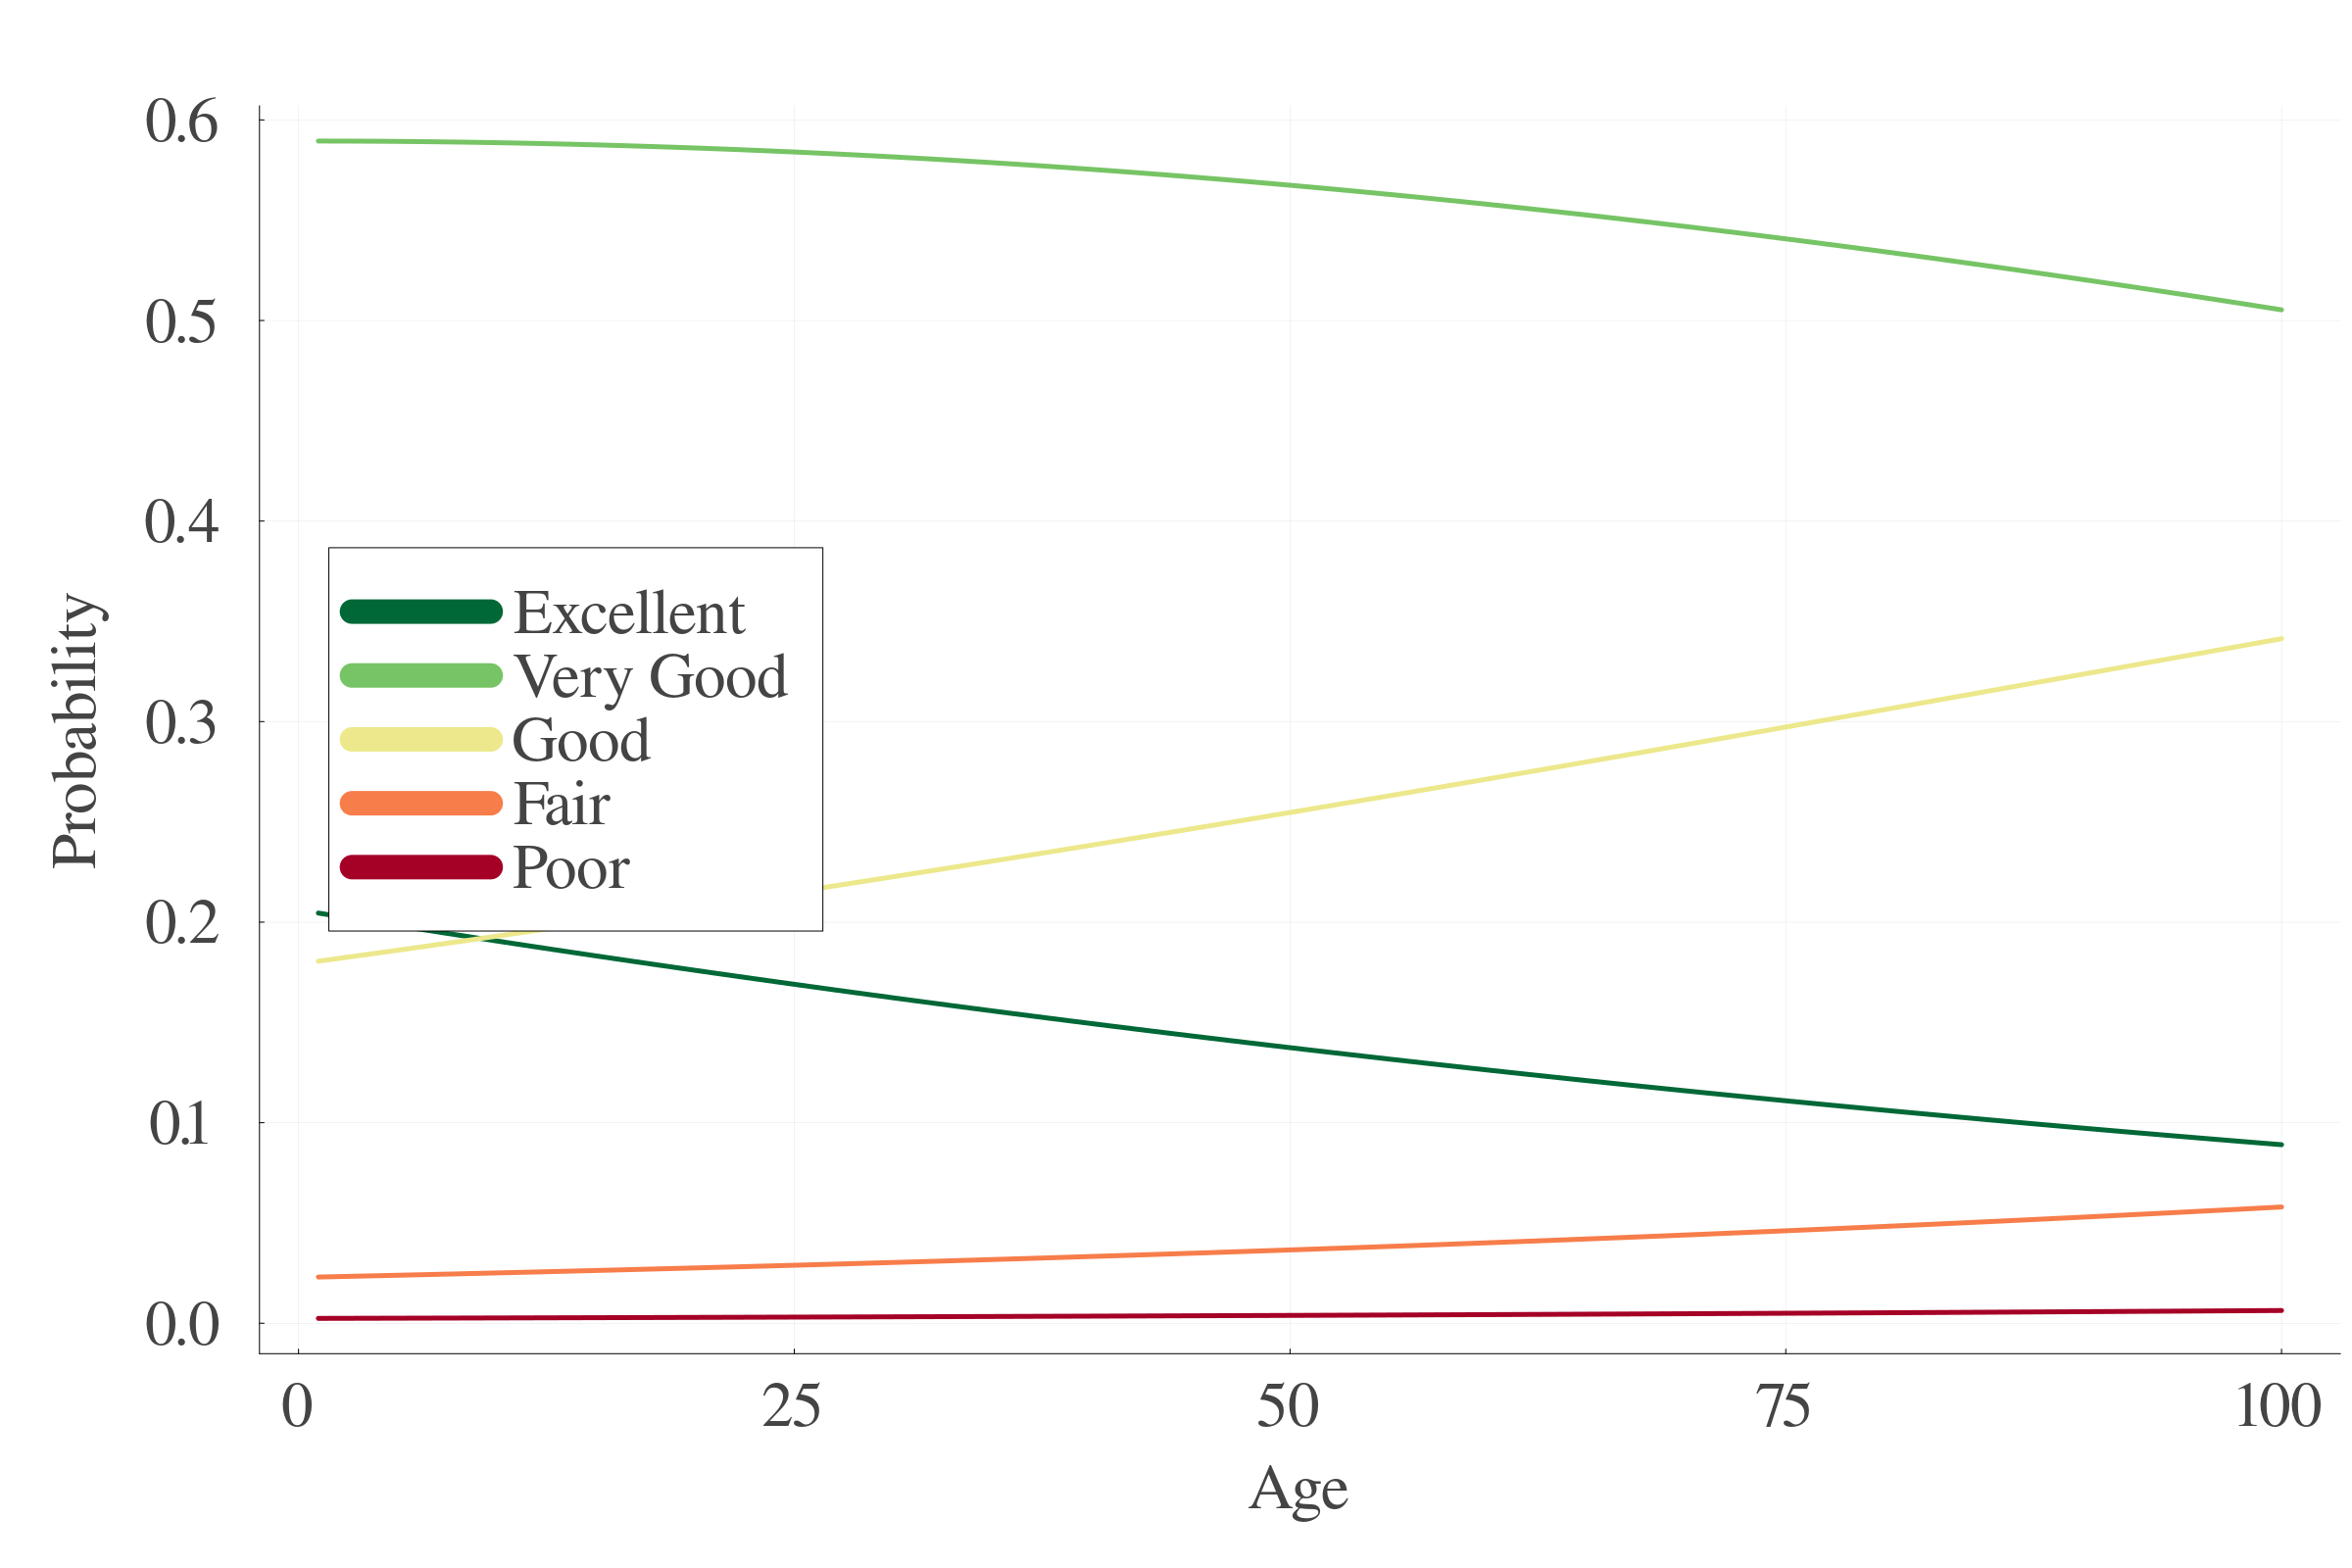
\includegraphics[width=\linewidth]{/Users/paulogcd/Documents/Master_Thesis/working_elements/Draft/output/health_transition_2.png}
    \caption{Transition probabilities from Very Good Health}
    \label{fig:sfig2}
    \end{subfigure}
    \begin{subfigure}{.5\textwidth}
    \centering
    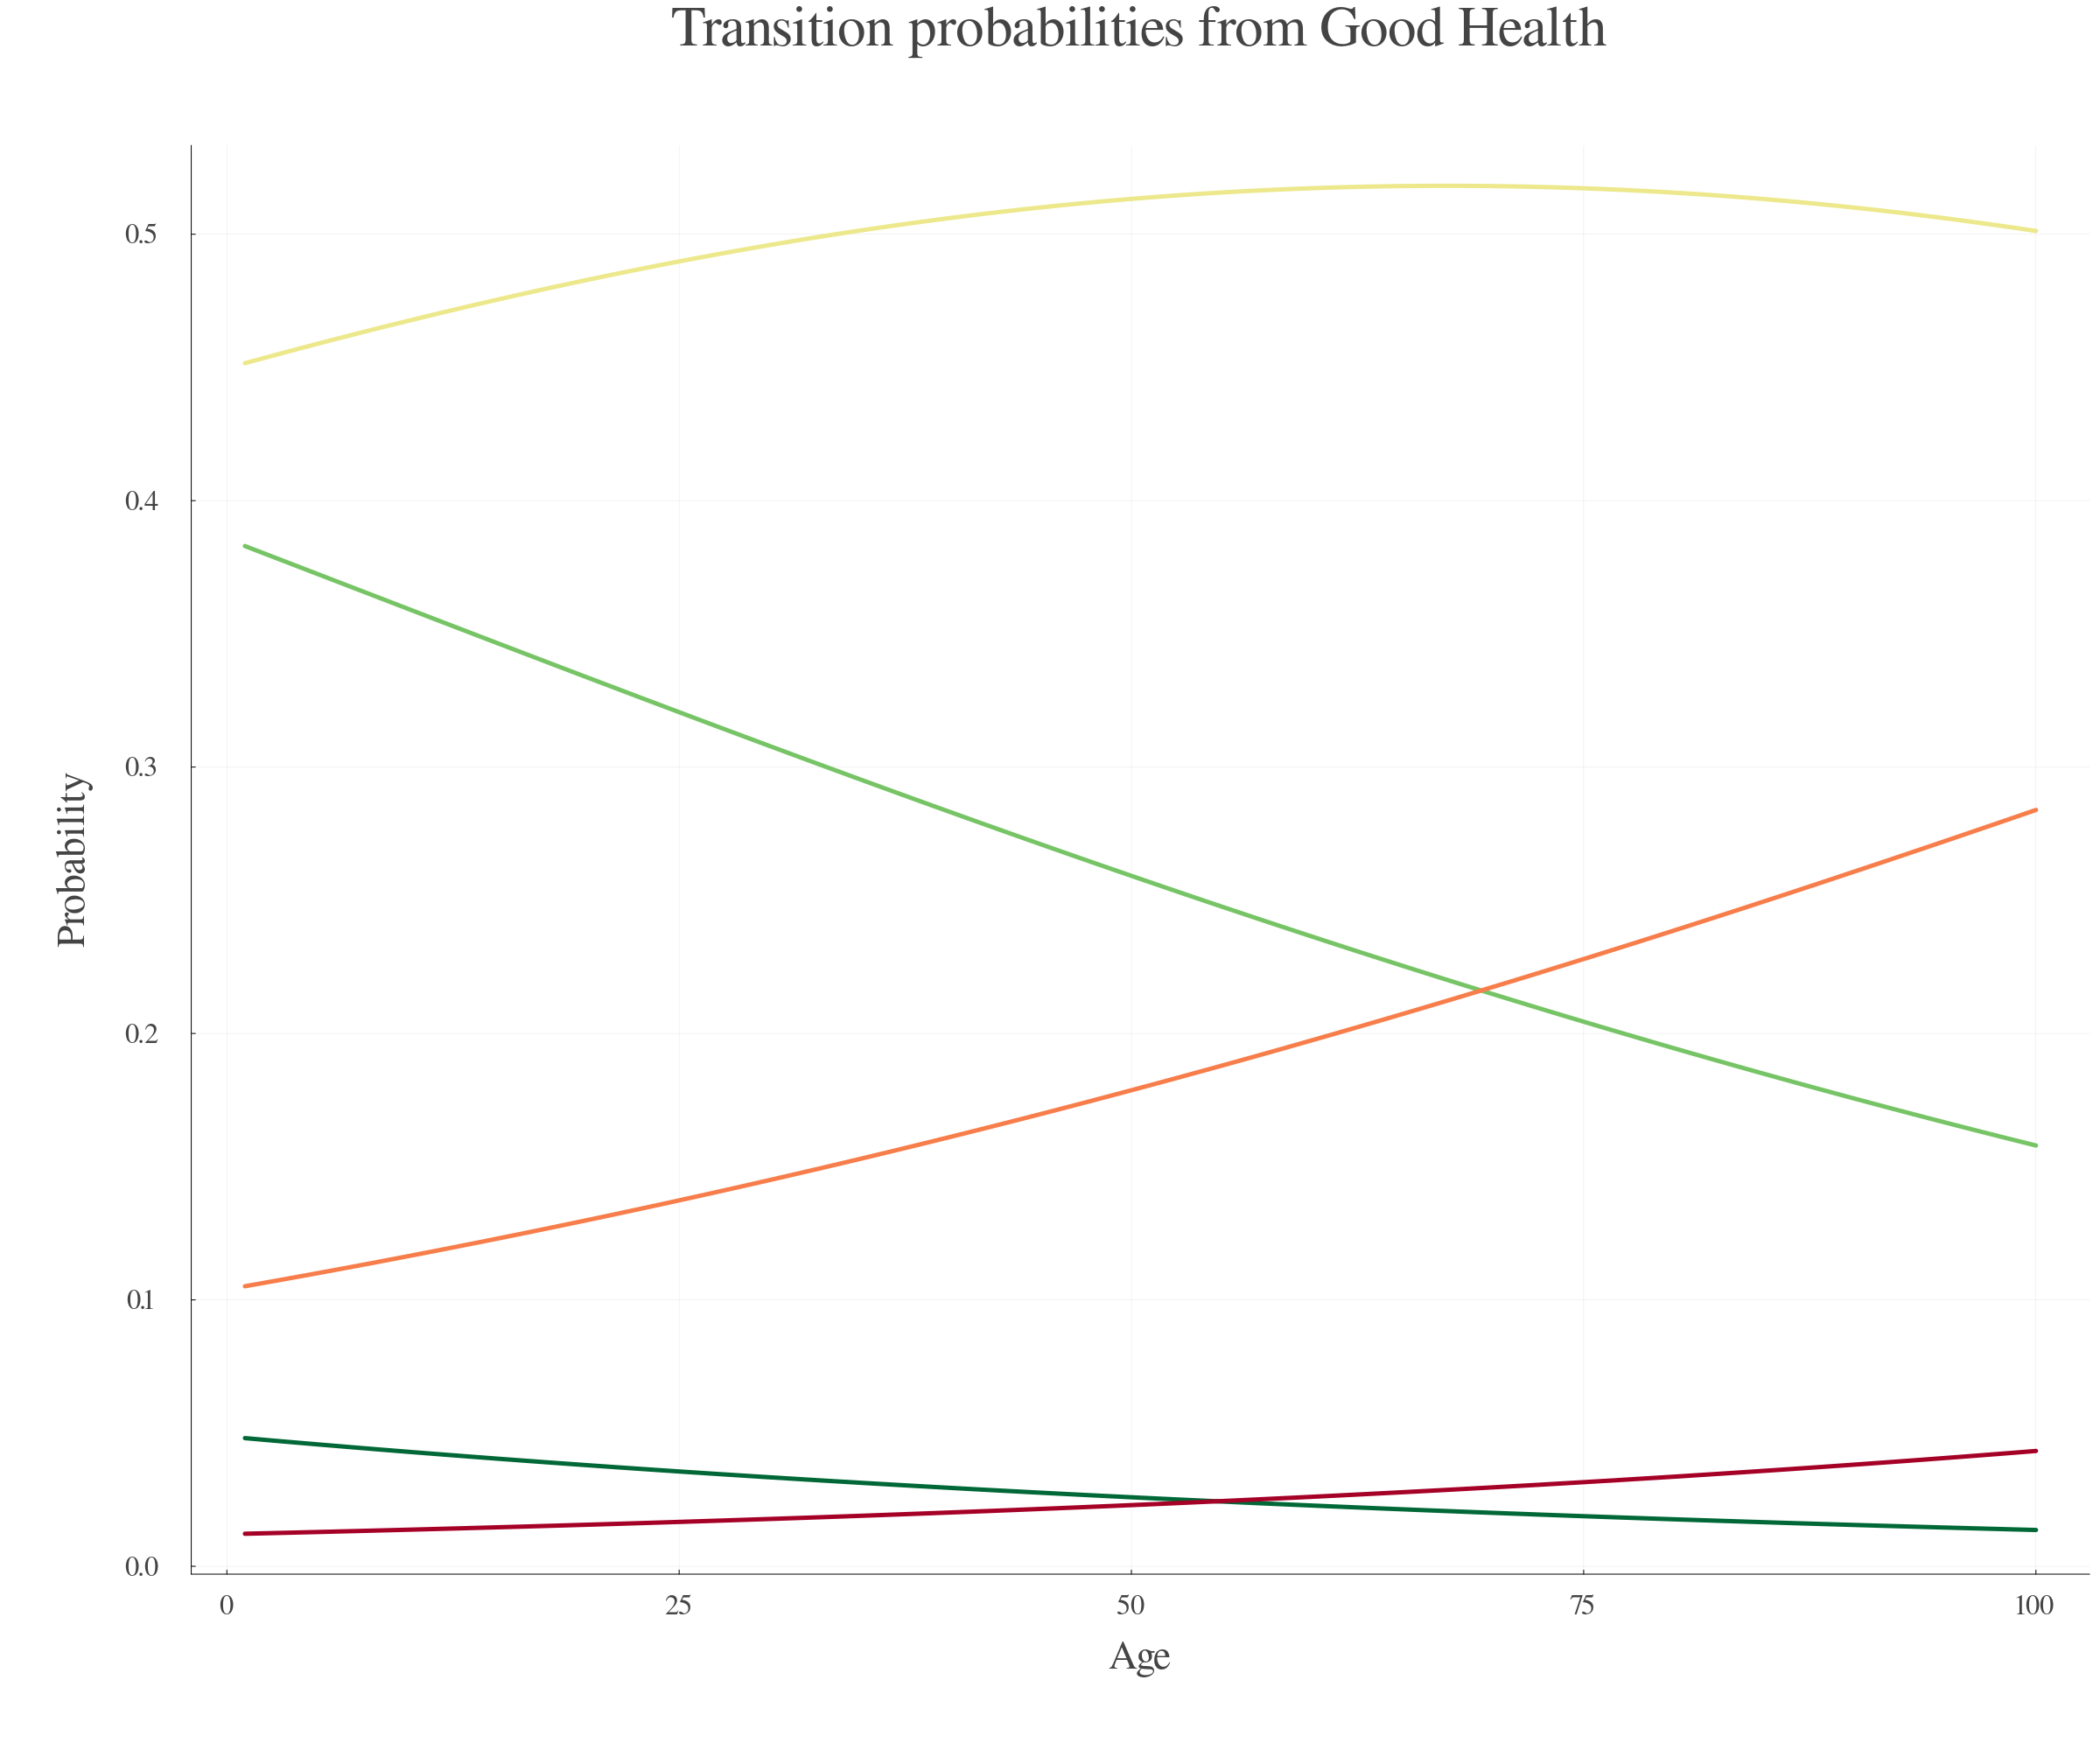
\includegraphics[width=\linewidth]{/Users/paulogcd/Documents/Master_Thesis/working_elements/Draft/output/health_transition_3.png}
    \caption{Transition probabilities from Good Health}
    \label{fig:sfig3}
    \end{subfigure}
    \begin{subfigure}{.5\textwidth}
    \centering
    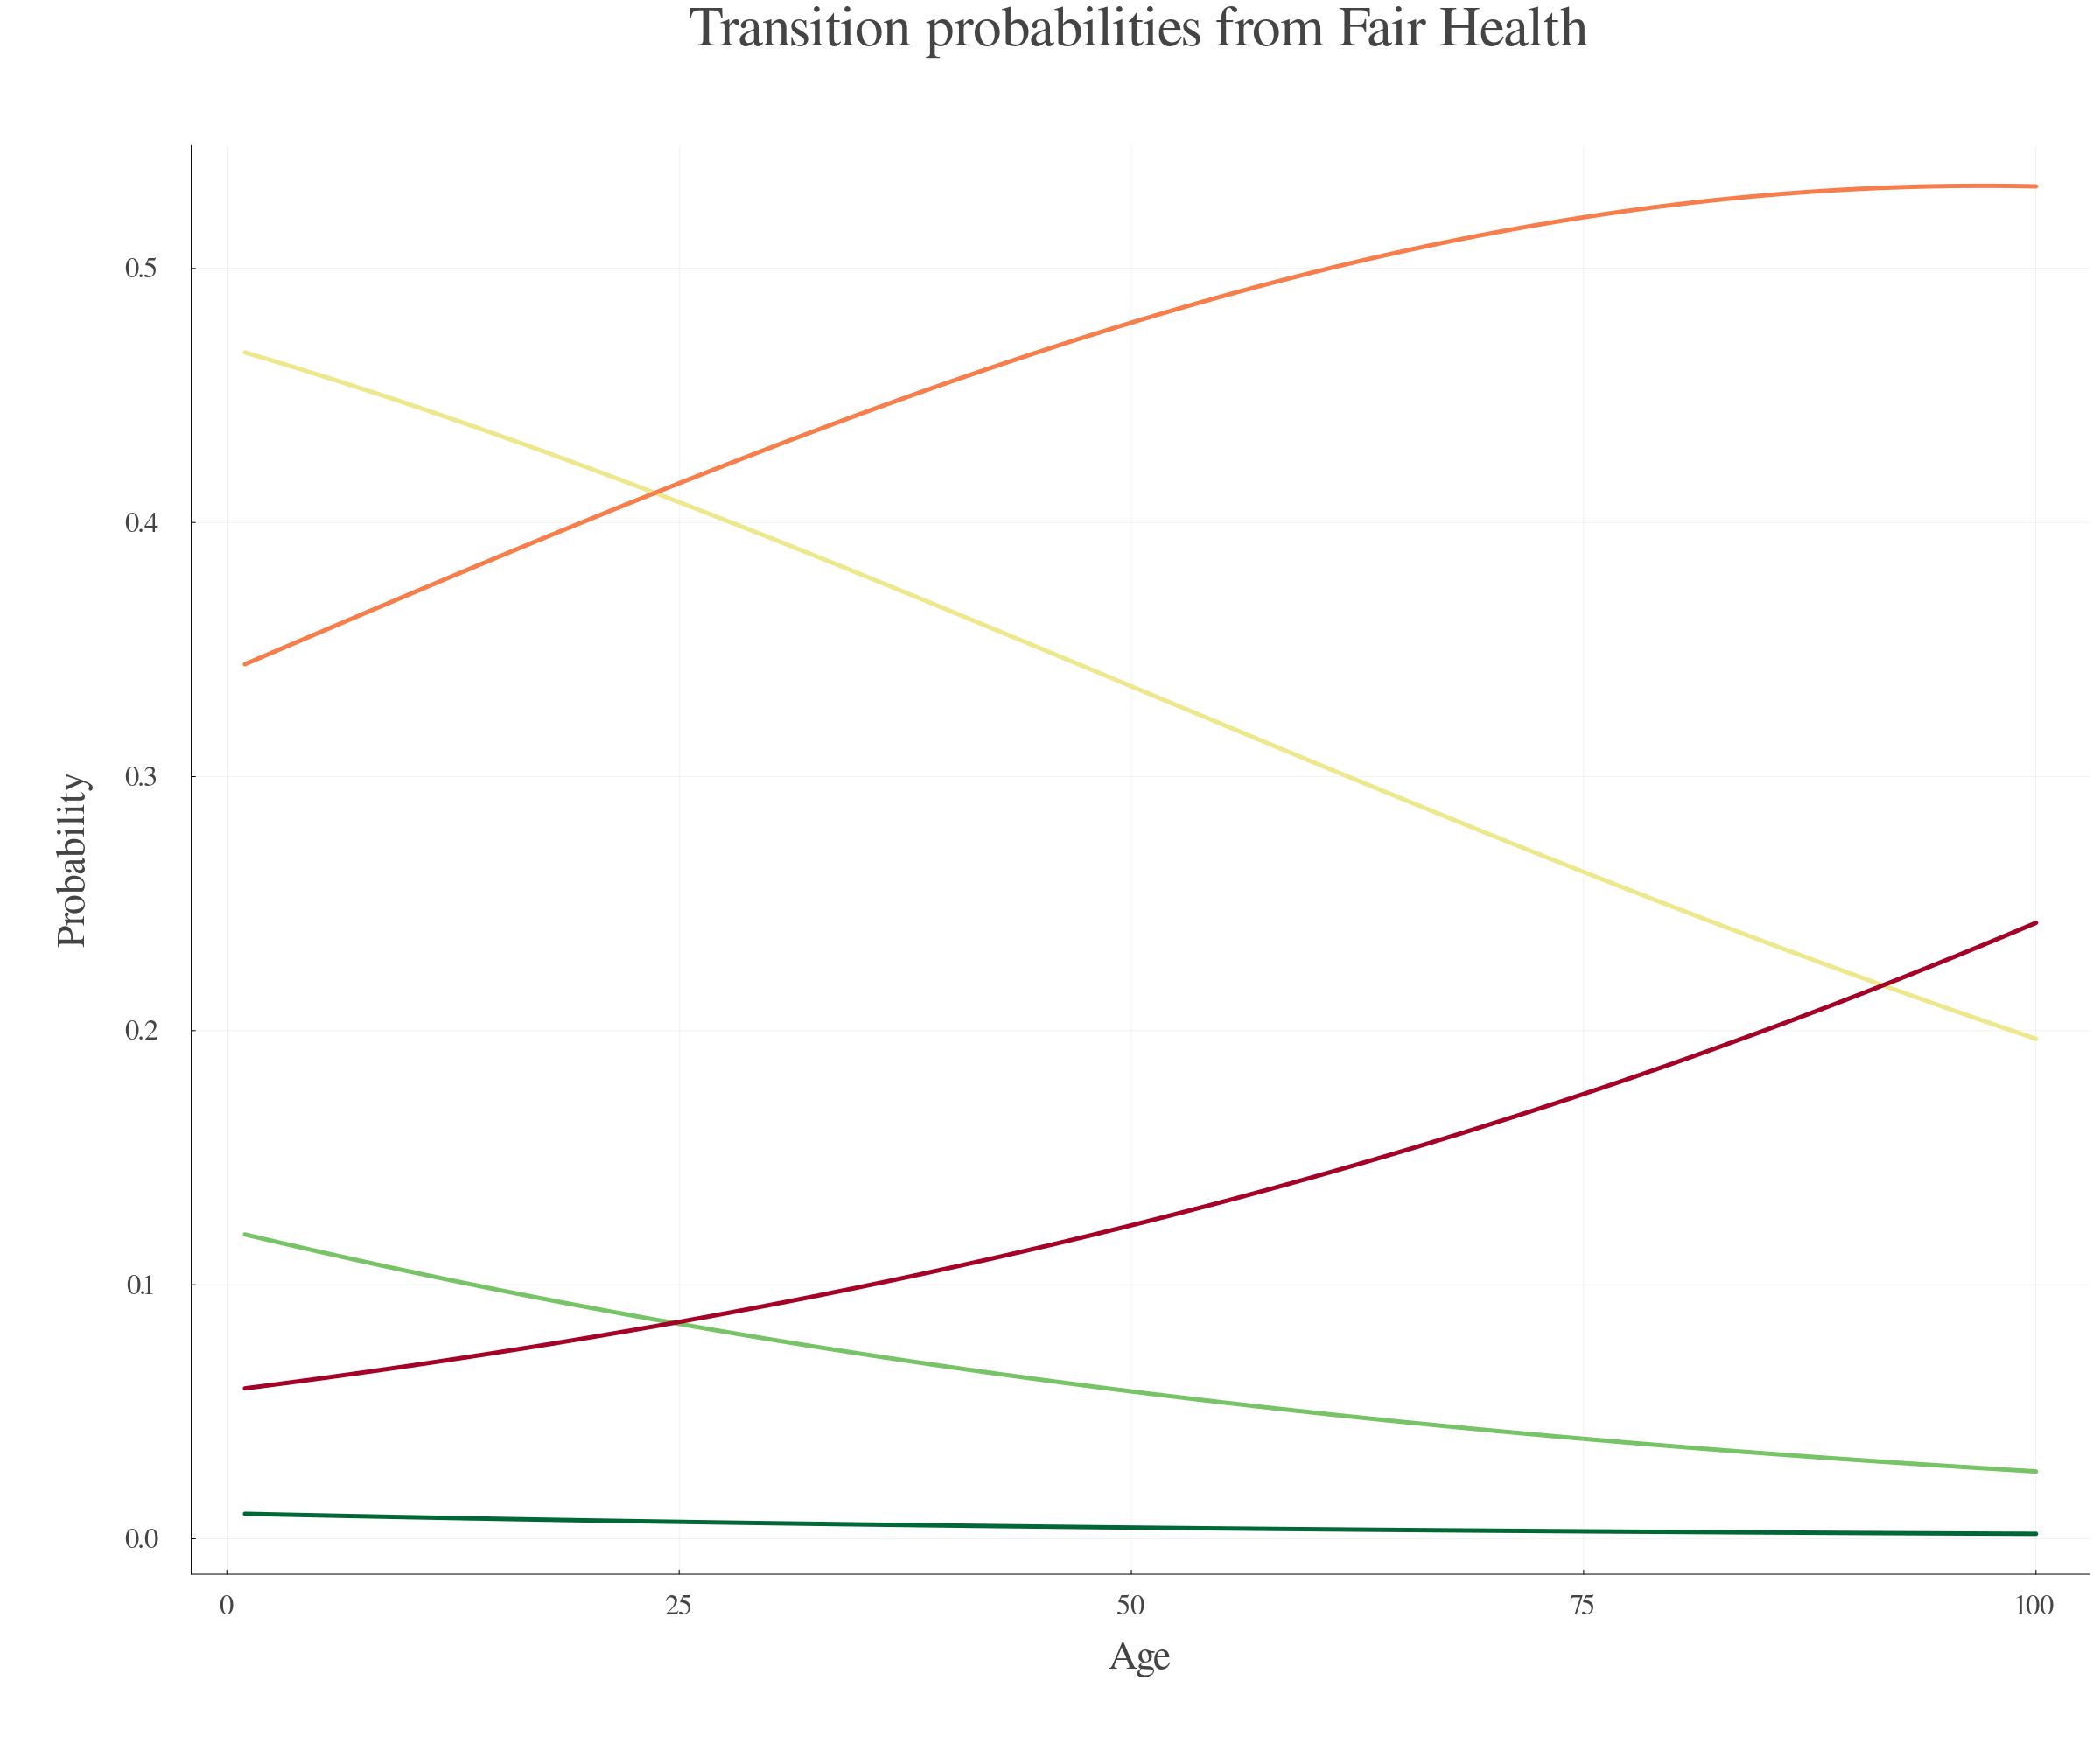
\includegraphics[width=\linewidth]{/Users/paulogcd/Documents/Master_Thesis/working_elements/Draft/output/health_transition_4.png}
    \caption{Transition probabilities from Fair Health}
    \label{fig:sfig4}
    \end{subfigure}
    \begin{subfigure}{.5\textwidth}
    \centering
    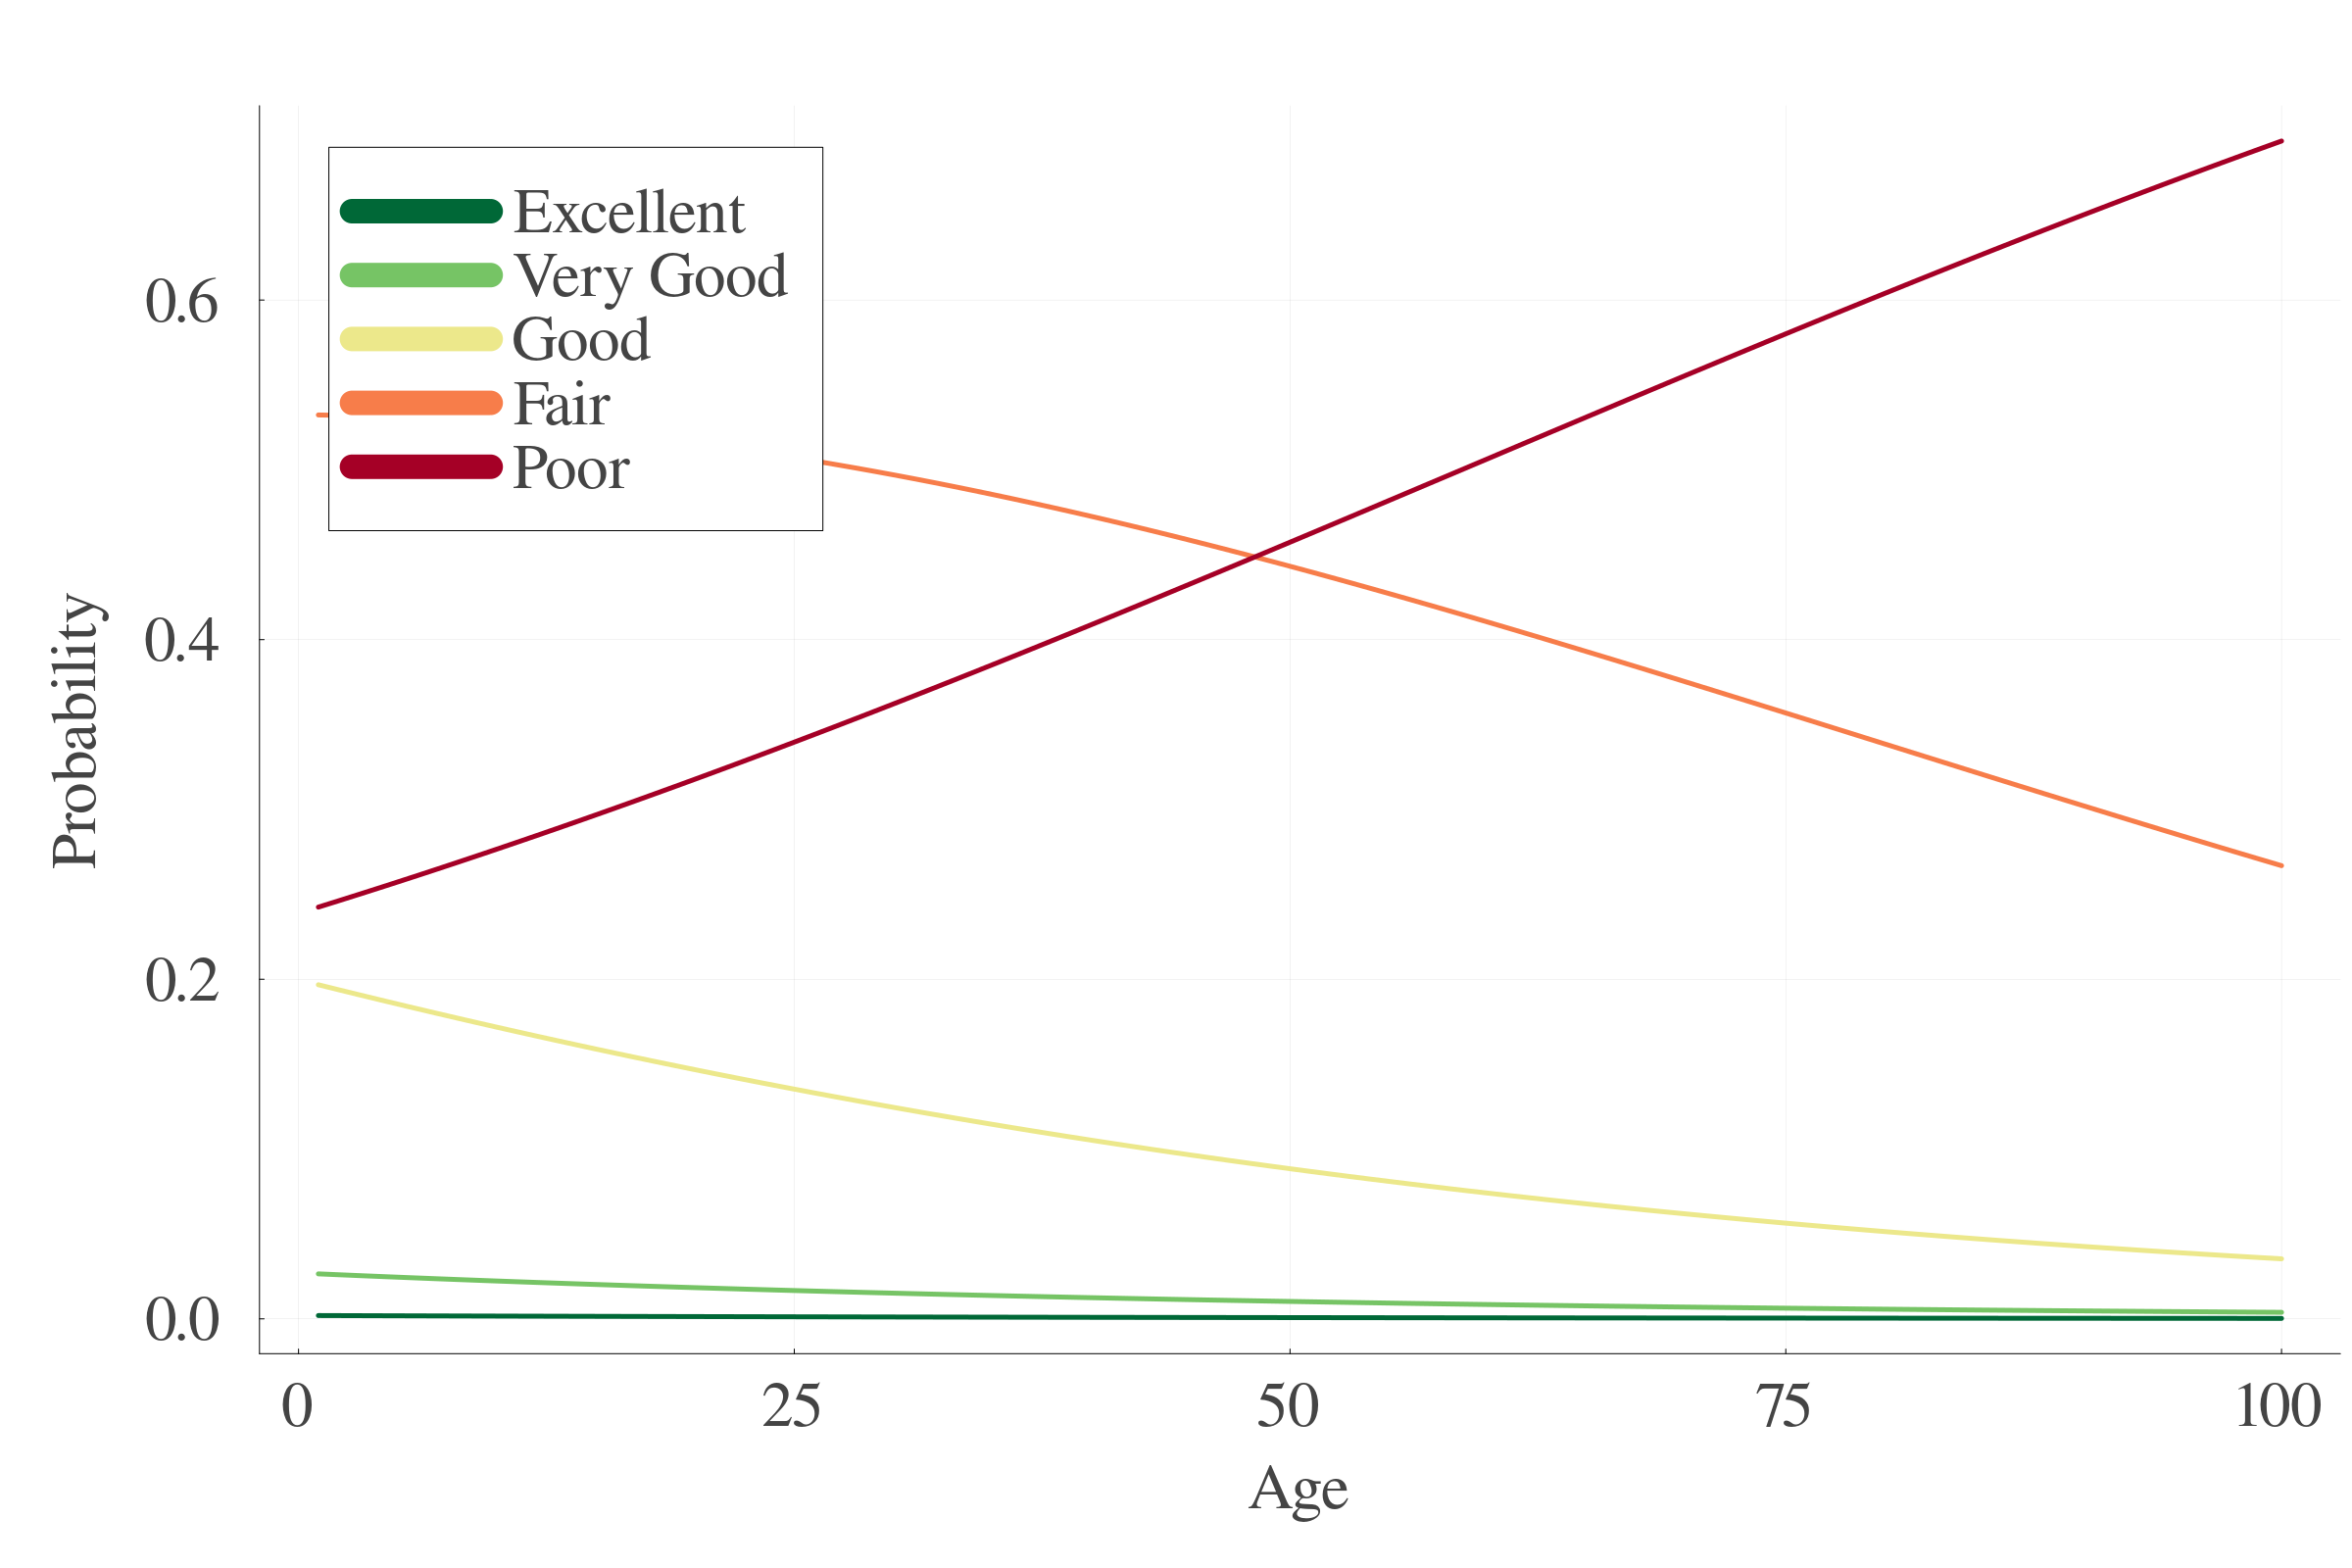
\includegraphics[width=\linewidth]{/Users/paulogcd/Documents/Master_Thesis/working_elements/Draft/output/health_transition_5.png}
    \caption{Transition probabilities from Poor Health}
    \label{fig:sfig2}
    \end{subfigure}
    \caption{Transition probabilities }
\end{figure}

From these estimates, it is possible to simulate the collective 
health trajectory of a population.

\begin{figure}[H]
    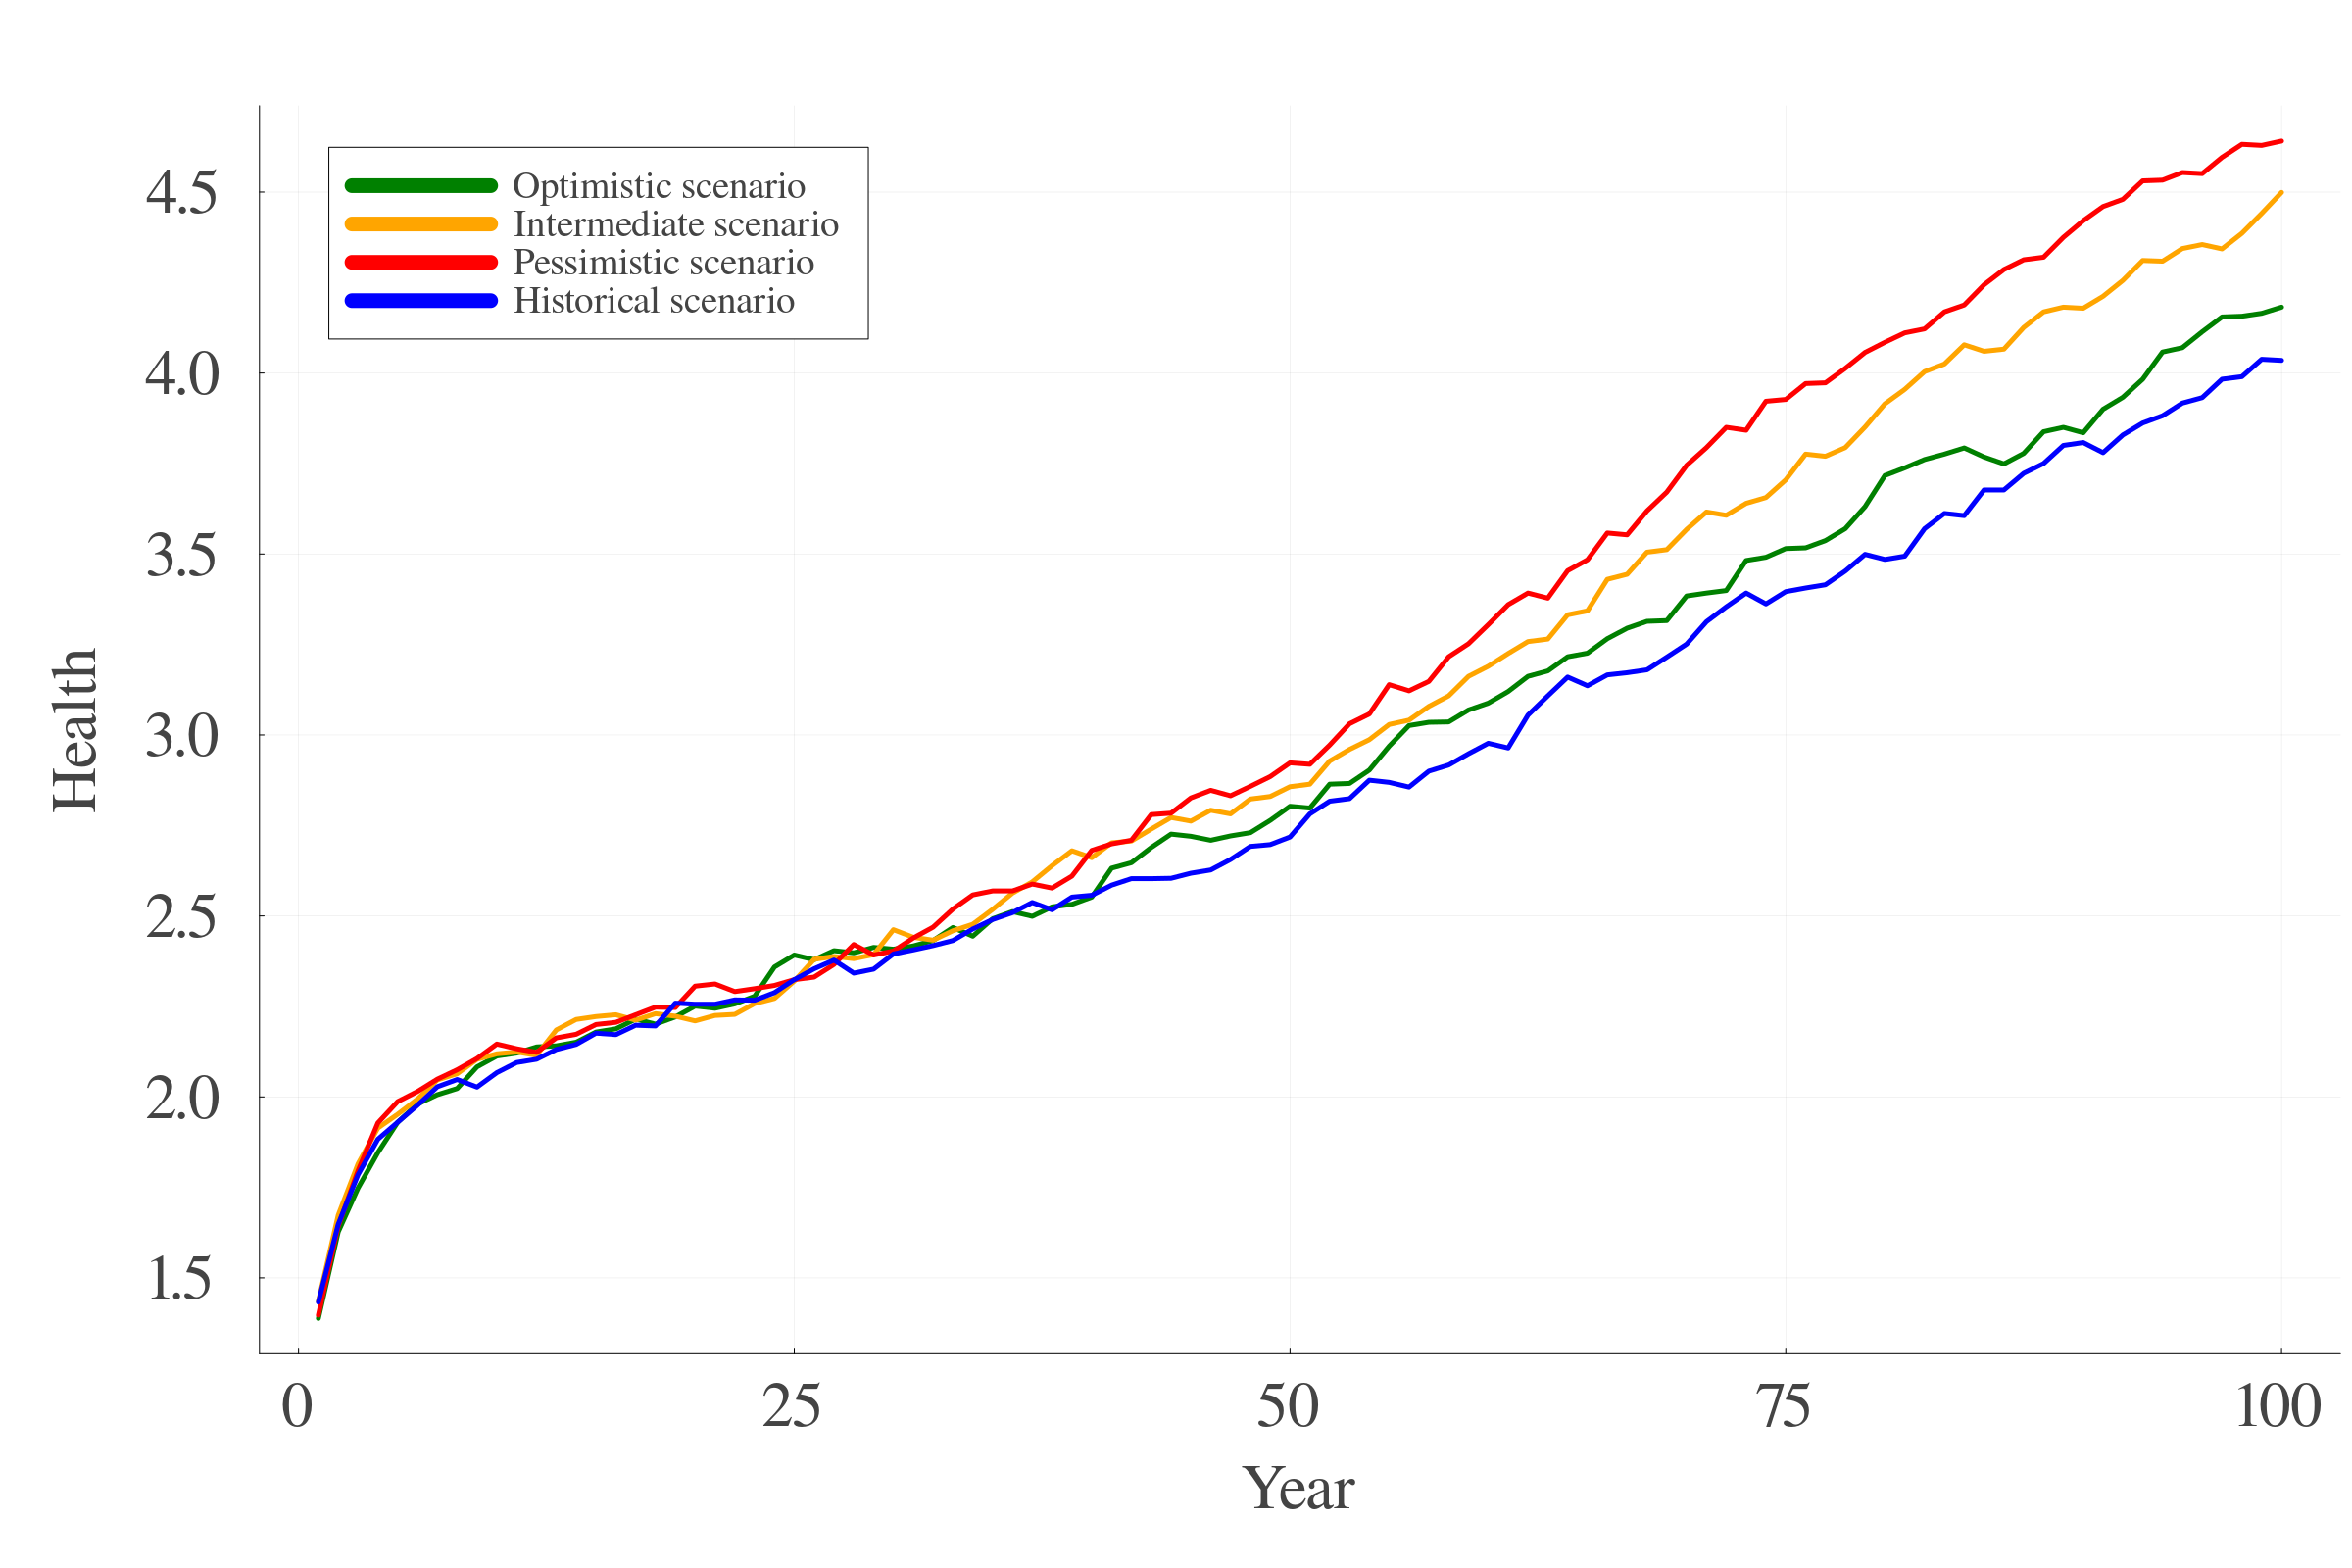
\includegraphics[width=\textwidth]{/Users/paulogcd/Documents/Master_Thesis/working_elements/Draft/output/average_health.png}
    \caption{Annual average health status as a function of temperature scenarios.}
\end{figure}

\subsubsection{Survival}

When taking into account the health transition estimates
and the survival probability estimates, it is then possible
to visualize the demographic evolution of a population through time.

\begin{figure}[H]
    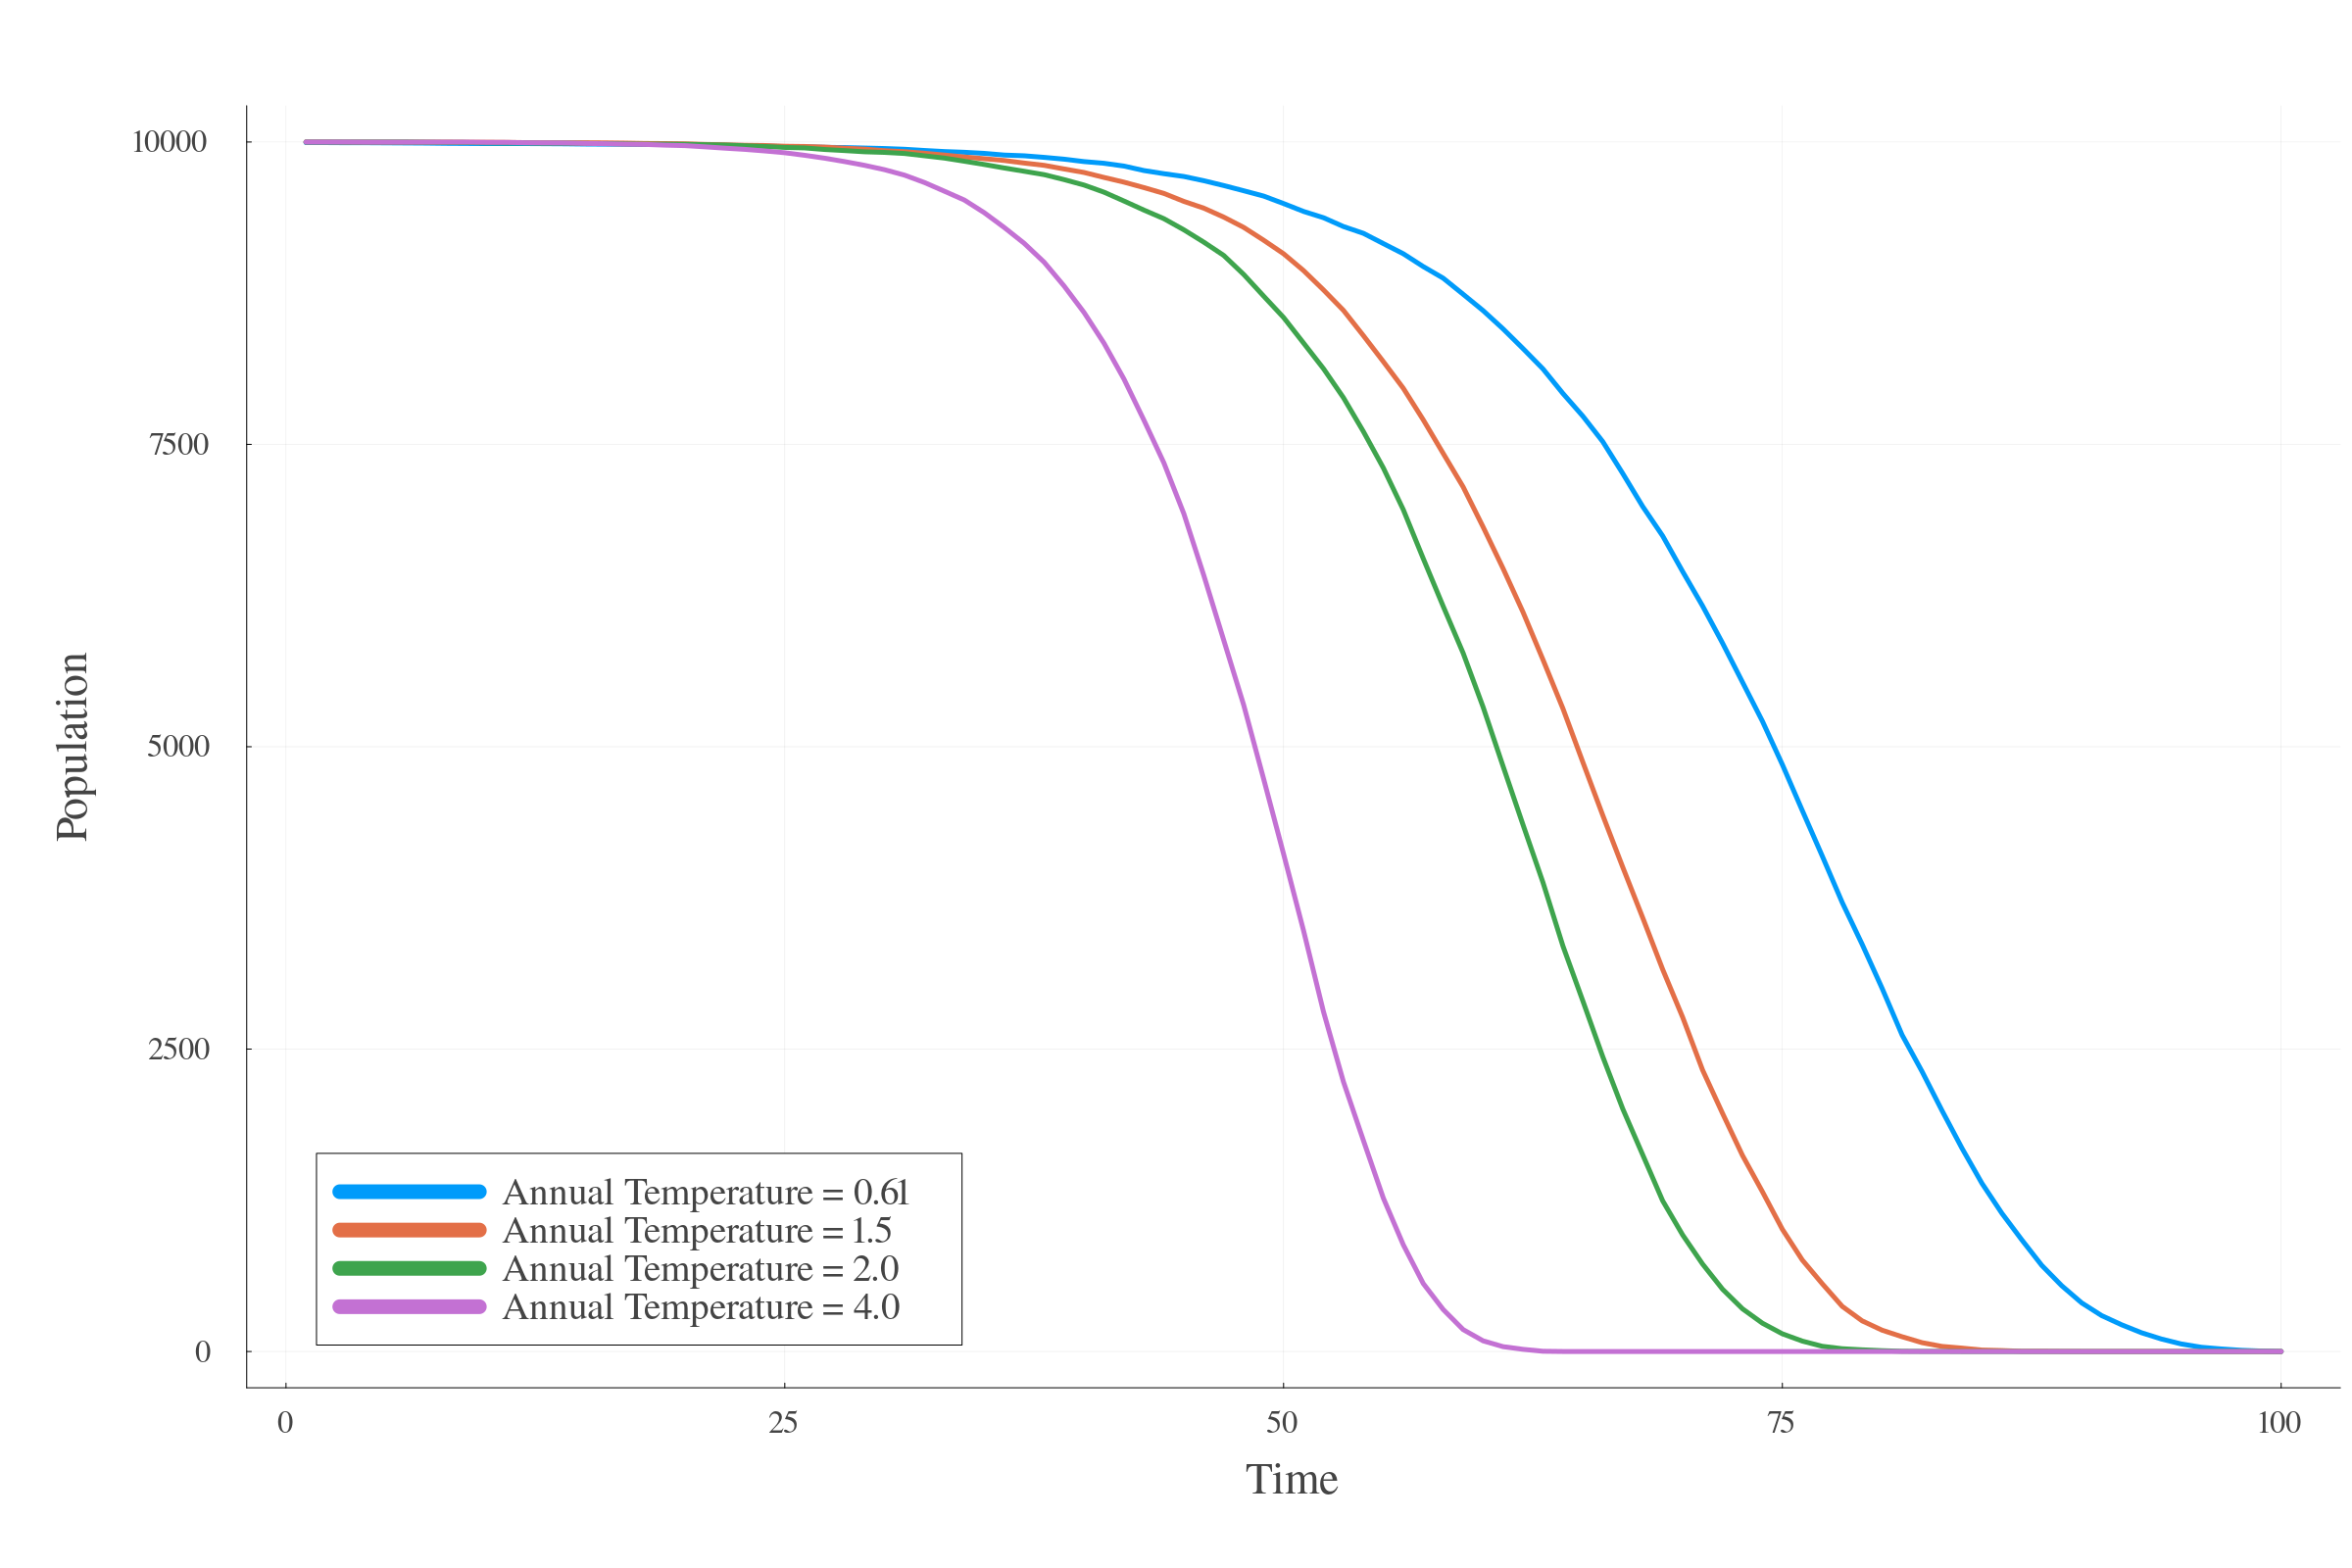
\includegraphics[width=\textwidth]{/Users/paulogcd/Documents/Master_Thesis/working_elements/Draft/output/figure_3.png}
    \caption{Annual probability of survival as a function of age and health status, obtained with $N_0$ =10 000 }
\end{figure}

\begin{table}[H]
    \begin{center}
        \begin{tabular}{cc}
            \toprule
            $\text{Temperature}$ & $\text{Life expectancy}$\\
            \midrule
            $4.0$ & $48.0$\\
            $2.0$ & $59.86$\\
            $1.5$ & $63.95$\\
            $0.61$ & $73.26$\\
            $0.5 - 4$ & $57.33$\\
            $0.5 - 2$ & $64.83$\\
            $0.0 - 1.5$ & $69.29$\\
            \bottomrule
        \end{tabular}
        \caption{Life expectancy simulations with fixed and variable temperatures.}
    \end{center}
\end{table}

We see that the effect of temperature on life expectancy 
is negative. 
This is due to the double effect of temperature on 
health transition and on survival probability.

DISCUSSION

These estimates are now going to be used in 
the economic model.

\section{Model}

This section is dedicated to the formal description of 
the model, as well as its analytical analysis.
First, its main mechanisms will be explained, and then, the 
inexistence of analytical solution in most cases will be shown.

\subsection{Baseline specification }

The agents maximizes: 

$$ \max_{\{c_{t},l_{t},s_{t+1}\}_{t=1}^{100}}{\mathbb{E}\left[\sum_{t=1}^{100} \beta^{t}\cdot u(c_t,l_t)\right]}$$

Their utility function is: 

$$u(c_{t},l_{t}) = \frac{c_{t}^{1-\rho}}{1-\rho}-\xi_{t}\cdot \frac{l_{t}^{1+\varphi}}{1+\varphi}$$

With : 

-  $c_{t}$  the consumption

-  $l_{t}$  the quantity of labor supply provided by the agent

-  $h_{t}$  the health status

-  $w_{t}$  the weather variable, which is here temperature

-  $\xi_{t}$ the labor disutility coefficient

- $\rho$ the risk aversion coefficient

- $\varphi$ the Frisch elasticity
\\

The agent is subject to the following budget constraint:

$$c_{t} + s_{t+1} \leq l_{t}\cdot z_{t} + s_{t}\cdot(1+r_{t})$$

With: 

-  $c_t$ the consumption at period $t$

-  $s_{t+1}$ the savings for period $t+1$

-  $l_t$ the labor supply provided by the agent at period $t$

-  $z_t$ the productivity at time $t$

-  $s_{t}$ the savings available at the beginning of period $t$

-  $r_{t}$ the interest rate at period $t$

Also, agents are subject to the following borrowing constraint, defined as: 

$$s_{t+1}\geq \underline{s}, \forall t \in [\![1,T]\!]$$


We can note the First Order Conditions, such that: 

\begin{equation}
    c^{-\rho}_{t}\cdot z_{t} = \xi_{t}\cdot l_{t}^{\varphi} \iff
        \begin{cases}
        & c_t = \left[\frac{\xi_{t}\cdot l_{t}^{\varphi}}{z_{t}}\right]^{-\frac{1}{\rho}}\\ 
        & l_{t} = \left[\frac{c_{t}^{-\rho}z_{t}\cdot}{\xi_{t}}\right]^{\frac{1}{\rho}}
    \end{cases}
\end{equation}
And 
\begin{equation}
    c^{-\rho}_{t} = \beta \cdot \mathbb{E}\left[c^{-\rho}_{t+1}\cdot (1+r_{t+1})\right] + \gamma_{t}
\end{equation}

The first corresponds to the equalization of marginal benefit and
cost of labor, and the second corresponds to the Euler equation.

The first equilbrium condition implies an within decision,
driven by the labor disutility coefficient $\xi$ and the productivity $z$.
There is a unique mapping between consumption and labor at any period, to 
equalize the benefits and the costs of labor.

The second equilibrium condition implies an intertemporal decision.
The marginal utility of consumption at one period must be equal to the 
expected marginal utility of conusmption next period, discounted by 
the discounting factor $\beta$ and the interest rate next period $(1+r_{t+1})$, 
plus the marginal benefit of violating the borrowing constraint at the current period. 

It is now important to describe what the Expectation operator $\mathbb{E}$ entails here. 
In a generic formulation, one could expect the uncertainty to affect the interest rate at the next period, 
which is the reason $(1+r_{t+1})$ is within the operator.

Another specification could exclude any uncertainty from 
the interest rate. 
The uncertainty could then come from the health and survival draw. 
If the uncertainty only comes from these two draws, the expectation operator can be formalized such as: 

$$\mathbb{E}\left[c_{t+1}\right] \equiv p_{t+1}(\mathcal{H}_{t},\mathcal{W}_{t}) \cdot c_{t+1}$$

In this specification, the only uncertainty is whether the agent will be alive or not in next period.
The baseline model will first focus on this simplified assumption. 
Variations will be introduced later.

\subsection{Analytical Solution Inexistence}

\textbf{Proposition}
This maximization program is impossible to solve analytically in most cases\footnote{The proof of this proposition is in the Appendix.}.
\\

If we consider the model altogether, it is impossible to describe 
analytically the optimal policy functions of the three choice variables.
While the entire proof is available in the appendix, a quick explanation
is possible here.
First, the objective functions is linear with the savings at next period $s_{t+1}$, 
making it disappear from the F.O.C.s.
This term requires therefore the labor and consumption policies to be solved, 
and then plugged into the budget constraint, to have a solution. 
However, if we try to solve the two other policy functions, 
we end up with transcendantal equations of the form $a\cdot x^{\alpha} + b\cdot x + c = 0$, 
with $\alpha\notin \mathbb{N}$. 
This transcendantal equations can be overcome with specific combinations 
of parameters, among which $\varphi = -\rho$, in which case we obtain: 

$$EQUATION$$

To allow for more flexibility in the resolution, the model was mainly solved
numerically.
The next section discusses the different methods used in order to do so.

\section{Numerical methods}

Several ways have been considered to solve this model numerically. 
This section is dedicated to the presentation of the different methods
used in order to do so. 
First, the auxiliary functions are presented. 
Second, the different main algorithms specifications and their performance are presented. 
Finally, the aggregation methods and different numerical results are discussed.

\subsection{Functions}

To proceed to a numerical solving of the model,  
some fundamental functions were used.

\begin{itemize}
    \item \textbf{Budget clearing function: } 
    The budget clearing function computes the amount of non used income for a 
    set of state and choice variables. Since at optimal, the budget constraint is binding, 
    the underlying theoreical result indicates that the budget clearing function should be 
    zero. Given the imprecision of numerical methods, the average budget clearing function was used 
    as a measure of the precision performance of each algorithm.

    It is equal to: 
    $$B(s_{t},l_{t},c_{t},s_{t+1})=l_{t} \cdot z_{t} + s_{t}\cdot(1+r_{t}) - s_{t+1} - c_{t}$$

    \item \textbf{Bellman function: }
    The Bellman function takes as an argument the value function next period, 
    and maximizes the current utility plus the discounted value function next period. 

    It is equal to: 
    $$V(s_{t}) = \max_{\{c_{t},l_{t},s_{t+1}\}\in \Gamma(s_{t})} \{u(c_{t},l_{t}) + \beta \cdot V(s_{t+1})\}$$
    With $\Gamma(s_{t})$ the feasibility set given by the state variable $s_{t}$.

    \item \textbf{Backwards function: }
    The backwards function iterates the Bellman function from the last period 
    to the first one. In the case of policy iteration, it iterates over the 
    policy function, and not the value function. It aggregates the optimal decisions 
    and returns a grid of optimal choices associated to each period and state variable value.

    For the pure numerical value function iteration, the backwards function is
    as following: 
    \begin{lstlisting}
for t from 100 to 1

    if t is equal to 100
        Bellman next period = Vector of zeros
    end

    for s in the possible set of s
        for c,l,s' in the feasible set of the current s value
            
            # We compute the budget clearing: 

            bc = budget_clearing(c,l,s') 

            # If it does not,
            # we set the value function to a very low number.
            
            if bc < 0

                V[c,l,s',s] = -Inf 
            
            # If it does, we compute the value function 
            # for this combination of choice variables.
            
            else if bc >= 0

                V[c,l,s',s] =
                    utility(c,l,s') +
                    beta * probability of survival *
                    Bellman next period[s']
            end
        end
        
        # We set the value function for s and t to
        # the maximum value found.
        
    end

# We set the value function at next period to current one
Bellman_next_period = Value_function[index_s,t]

end
\end{lstlisting}

\end{itemize}


\subsection{Algorithms}

This section details the different algorithms
developed to perform a numerical 
solution of the model. 

\subsubsection{Pure numerical value function iteration}

The pure numerical value function iteration algorithm consists
in verifying all possible 
combination of choice variables for each level of state variable 
to determine what is the best possible response given a certain
amount of state variable \footnote{The different steps of the algorithms and their source code are available online.
The steps and comments of the present work are available here: \url{https://www.paulogcd.com/Master_Thesis/},
and the documented replication package, coded in Julia, is available here: \url{https://www.paulogcd.com/Master_Thesis_Paulogcd_2025/}.}.

Here, the algorithm goes through all the possible values of
$c$, $l$, and $s'$, without using any approximation obtained 
through the FOC mentioned above. 
This is quite computational-intensive, but 
has the advantage of not using analytical results, 
which can lead to approximation depending on the resolution of the 
ranges used.

\subsubsection{F.O.C. approximated value function iteration}

The FOC value function iteration algorithms
make use of the two FOC
derived in the previous section. 
They are faster by order of magnitudes,
but contain more errors.

Note that it is impossible to use the second FOC, i.e. the 
Euler equation, containing the 
Lagrangien multiplier $\gamma_{t}$ that
is not solvable analytically. 

\subsubsection{Interpolated algorithms}

The interpolated algorithms 
use interpolation techniques to approximate 
the value of the next period Bellman equation. 
This interpolation can be implemented in the pure numerical 
algorithm, and in the FOC-approximated ones. 

They allow for a smoother shape of policy function, 
and are more easily graphically interpretable.
However, 
their results on speed
performance is slightly worse, 
and their results on precision
performance is ambiguous. 

\subsubsection{Policy iteration algorithms}

The policy iteration algorithms use a 
backward function iterating on the policy function, 
and not on the value function.

\section{Results}



\section{Conclusion}

\section{References}

\printbibliography

\newpage
\section{Appendix}

\subsection{Proof of Impossibility}

This section is dedicated to the proof that the maximization program
has no analytical solution in most cases.

We will show this absence of analytical solution by attempting to solve it in three different 
ways: First by using the Budget Constraint binding, then by using the F.O.C. and the Budget Constraint,
and lastly trying to go to the last period to solve it recursively. 

\subsubsection{Maximization program}

$$ \max_{\{c_{t},l_{t},s_{t+1}\}_{t=1}^{100}}
{\mathbb{E}\left[\sum_{t=1}^{100} \beta^{t}\cdot \frac{c_{t}^{1-\rho}}{1-\rho}-\xi_{t}\cdot \frac{l_{t}^{1+\varphi}}{1+\varphi}\right]}$$

Subject to budget and borrowing constraints:

$$c_{t} + s_{t+1} \leq l_{t}\cdot z_{t} + s_{t}\cdot(1+r_{t})$$

$$s_{t+1}\geq \underline{s}, \forall t \in [\![1,100]\!]$$

\subsubsection{Budget constraint binding}

A first solving attempt consists in assuming that the budget constraint binds.
We can then obtain the following expression for consumption: 

$$c_{t} = l_{t}\cdot z_{t} + s_{t}\cdot(1+r_{t}) - s_{t+1}$$

Plugging it into the maximization program, we obtain:

$$ \max_{\{l_{t},s_{t+1}\}_{t=1}^{100}}
{\mathbb{E}\left[\sum_{t=1}^{100} \beta^{t}\cdot \frac{\left(l_{t}\cdot z_{t} + s_{t}\cdot(1+r_{t}) - s_{t+1}\right)^{1-\rho}}{1-\rho}-\xi_{t}\cdot \frac{l_{t}^{1+\varphi}}{1+\varphi}\right]}$$

The F.O.C. with respect to labor implies: 

\begin{equation}
    l_{t}^{\varphi}\cdot \xi_{t} = \left[l_{t}\cdot z_{t} + s_{t}\cdot(1+r_{t})- s_{t+1}\right]^{-\rho}\cdot z_{t}
\end{equation}

We can develop the decomposition of consumption if and only if $\rho \in \mathbb{N}$.
Indeed, this equation is of form $x = (x-\alpha)^{\beta} \cdot z$.
With $\beta\notin \mathbb{N}$, is a transcendantal equation.

\subsubsection{F.O.C. and Budget clearing}

We can now try to compute the F.O.C. first, and then make use of the Budget Constraint.
The Lagrangien function associated witht the maximization program of the agent is: 
\begin{equation}
    \begin{split}
        \mathcal{L}(c_{t},l_{t},s_{t+1};\lambda_t,\gamma_{t}) &
        = \mathbb{E}\Big[\sum_{t=1}^{100} \beta^{t}\cdot ((\frac{c_{t}^{1-\rho}}{1-\rho}-\xi_{t}\cdot\frac{l_{t}^{1+\varphi}}{1+\varphi}) \\
        & +\lambda_{t}\cdot \left(l_{t}\cdot z_{t}+s_{t}\cdot (1+r_{t})-c_{t}-s_{t+1}\right) \\ 
        & + \gamma_{t}\cdot \left(s_{t+1}-\underline{s}\right))\Big] \\ 
    \end{split}
\end{equation}

The First Order Conditions are the following:

$$\frac{\partial \mathcal{L}}{\partial c_{t}} = 0 \iff c_{t}^{-\rho} = \lambda_{t}$$


$$\frac{\partial \mathcal{L}}{\partial l_{t}} = 0 \iff \lambda_{t}\cdot z_{t} = \xi_{t}\cdot l_{t}^{\varphi}$$


$$\frac{\partial \mathcal{L}}{\partial s_{t+1}} = 0 \iff \lambda_{t} = \beta \cdot \mathbb{E}\left[\lambda_{t+1}\cdot (1+r_{t+1})\right] + \gamma_{t}$$

We first note that we must obtain a closed-form solution for $c_{t}$ and $l_{t}$ to obtain 
the optimal value of $s_{t+1}$. 
Indeed, since $s_{t+1}$ is linear in $\mathcal{L}$, we would need to plug the closed-form
solutions of $c_{t}$ and $l_{t}$ in the budget constraint. \\

Replacing the expression of $\lambda_{t}$ in the two other equation yields: 

\begin{equation}
    c^{-\rho}_{t}\cdot z_{t} = \xi_{t}\cdot l_{t}^{\varphi} \iff
        \begin{cases}
        & c_t = \left[\frac{\xi_{t}\cdot l_{t}^{\varphi}}{z_{t}}\right]^{-\frac{1}{\rho}}\\ 
        & l_{t} = \left[\frac{c_{t}^{-\rho}z_{t}\cdot}{\xi_{t}}\right]^{\frac{1}{\rho}}
    \end{cases}
\end{equation}
And 
\begin{equation}
    c^{-\rho}_{t} = \beta \cdot \mathbb{E}\left[c^{-\rho}_{t+1}\cdot (1+r_{t+1})\right] + \gamma_{t}
\end{equation}

Assuming that the budget constraint binds, it becomes, as previously seen:

$$c_{t} + s_{t+1} = l_{t}\cdot z_{t} + s_{t}\cdot(1+r_{t})
\iff 
c_{t} = l_{t}\cdot z_{t} + s_{t}\cdot(1+r_{t}) - s_{t+1} 
$$

This leads to the following equation system: 

$$
\begin{cases}
    & c_t = \left[\frac{\xi_{t}\cdot l_{t}^{\varphi}}{z_{t}}\right]^{-\frac{1}{\rho}} \\
    & c_{t} = l_{t}\cdot z_{t} + s_{t}\cdot(1+r_{t}) - s_{t+1} 
\end{cases}
$$

$$\iff$$
$$ \left[\frac{\xi_{t}\cdot l_{t}^{\varphi}}{z_{t}}\right]^{-\frac{1}{\rho}} = l_{t}\cdot z_{t} + s_{t}\cdot(1+r_{t}) - s_{t+1} $$
$$\iff$$
$$ l_{t}^{-\frac{\varphi}{\rho}} \cdot \left(\frac{\xi_{t}}{z_{t}}\right)^{-\frac{1}{\rho}} = l_{t}\cdot z_{t} + s_{t}\cdot(1+r_{t}) - s_{t+1} $$
$$\iff$$
$$ l_{t}^{-\frac{\varphi}{\rho}} \cdot \left(\frac{z_{t}}{\xi_{t}}\right)^{\frac{1}{\rho}} - l_{t}\cdot z_{t} - s_{t}\cdot(1+r_{t}) - s_{t+1} = 0 $$

This is a transcendantal equation of form 
$x^{\alpha}\cdot b - x\cdot y - c = 0$,
which admits a solution if and only if $-\frac{\varphi}{\rho} \in \mathbb{N}$.
This condition seems unrealistic in our context: 

\begin{itemize}
    \item $-\varphi >0$ implies that labor has a decreasing disutility,
    which makes the maximization program absurd.
    \item $-\rho >0$ implies a risk-loving agent, which changes 
    drastically the framework of our model, and would require another whole 
    interpretation.
\end{itemize}

Note that if we set $-\rho\in\mathbb{N}$ and further develop the last equation in the 
budget constraint binding attempt, we end up with the same condition.

\subsubsection{Backwards solving attempt}

If we try to solve it backwards, we now go to the last period. 
At the last period, $s_{t+1} = \underline{s}$ for sure:
Since there is no future, 
the agent will borrow as much as they can,
or will at least not save anything more than what is imposed 
by the constraint. 

For simplification, let $\underline{s}$ be fixed such that: $\underline{s} = 0$.
The new optimality condition is: 

\begin{equation}
    l_{t}^{\varphi}\cdot \xi_{t} = \left[l_{t}\cdot z_{t} + s_{t}\cdot(1+r_{t})\right]^{-\rho}\cdot z_{t}
\end{equation}

Although we simplified the term at the exponential of which 
we have $-\rho$, this is still a transcendantal equation due to the sum 
of labor income and income coming from savings of last period, and the problem remain the same.

\end{document}